%!TEX root = ../slides.tex
\begin{frame}[noframenumbering]{Research background}{Contributions}
\small
\begin{block}{\small \textbf{Contributions}}
\begin{itemize}
  \item An on-device mobility patterns detector that works with streams of raw data collected by smartphone's sensors (GPS and accelerometer).
  \item An on-device mobility analyzer that incrementally builds a model of user mobility from the detected mobility patterns.
  \item A cognitive controller inspired on CDSs that, based on the mobility information learned, dynamically adapts GPS sampling rate through power-aware policies. 
  \item A middleware with the previous modules embedded for easing the development of LBSs and MBSs for the Android mobile platform.
\end{itemize}
\end{block}
\end{frame}

{\aauwavesbg%
  \begin{textblock*}{5cm}(0.3cm,0.3cm)
  \small
  \textbf{The architecture of the proposed system implemented in the Android software stack.}
  \end{textblock*}
% \begin{textblock*}{1cm}(12cm,9.3cm)
%   \scriptsize
%   \insertframenumber~/~\inserttotalframenumber
%   \end{textblock*}
\begin{frame}[plain,noframenumbering]
  \centering
  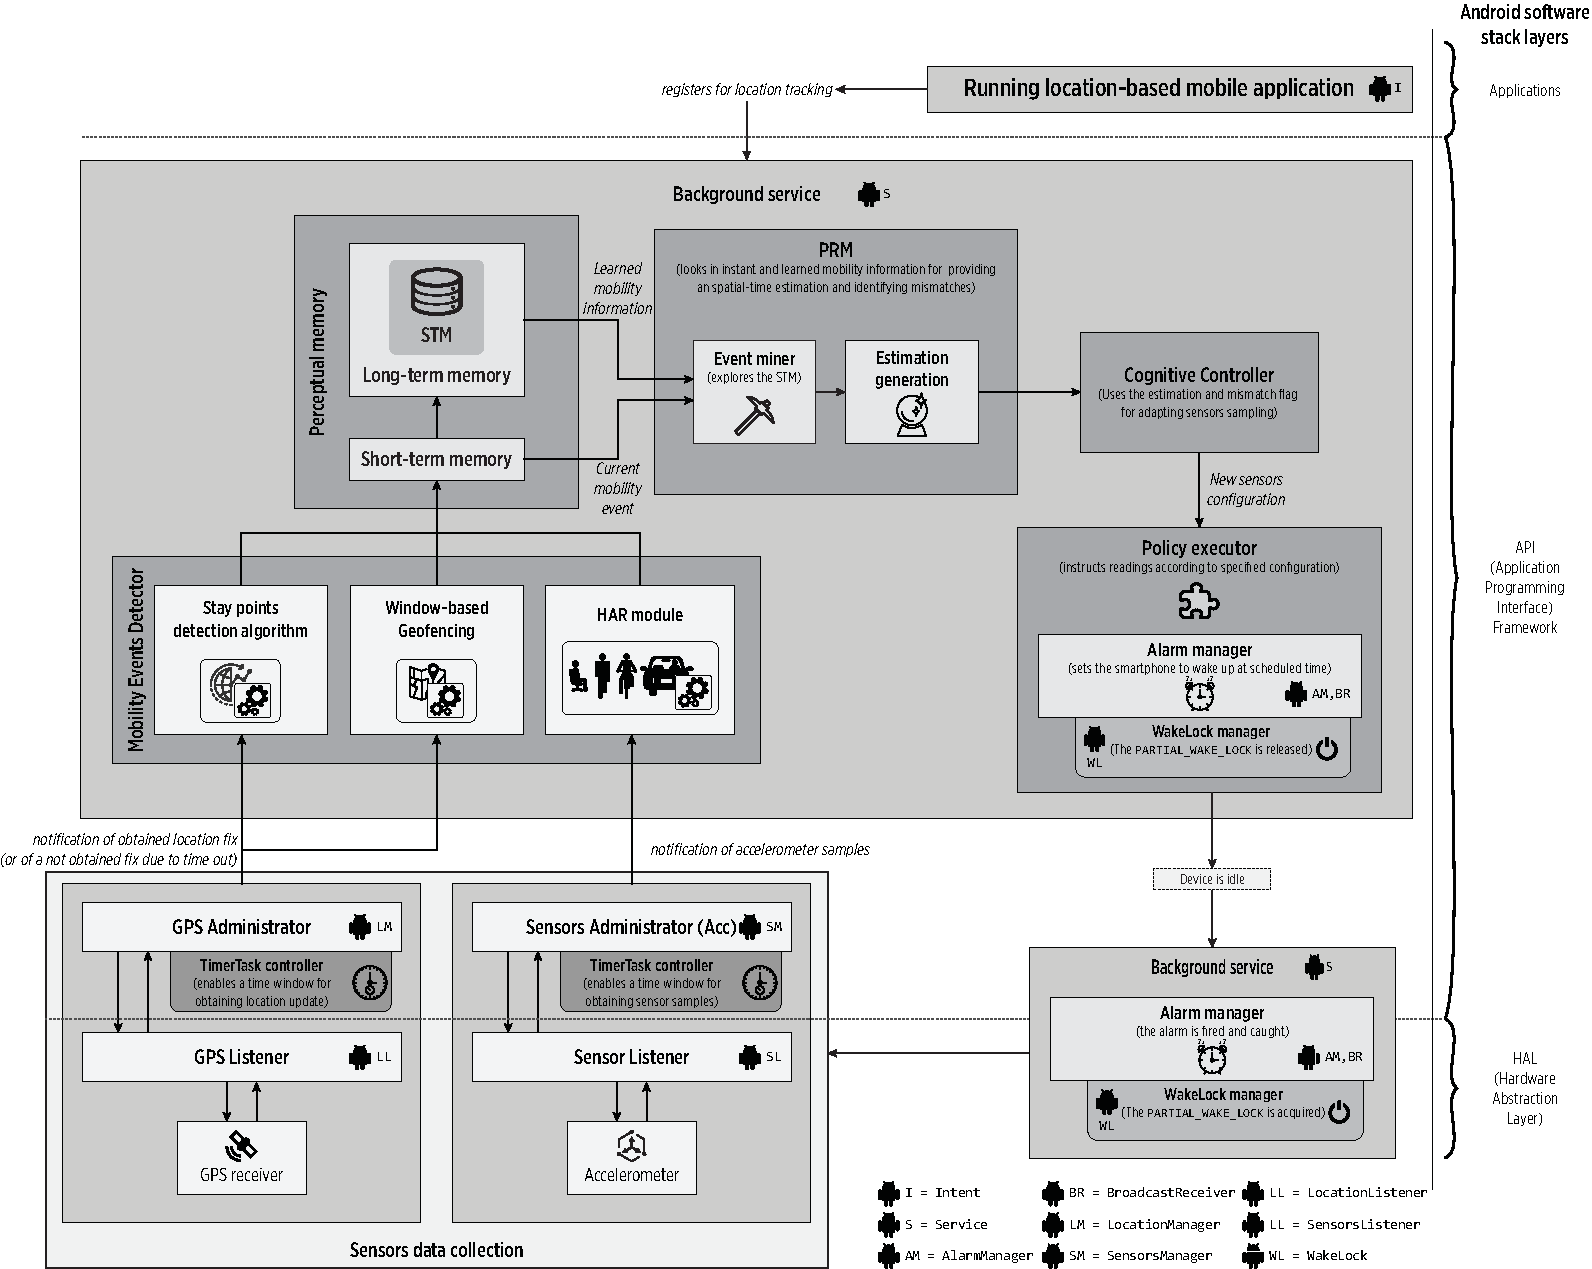
\includegraphics[width=\textwidth]{vectors/implementation}
\end{frame}}

\begin{frame}[noframenumbering]{Experimentation}{\emph{Stay Points Detector} module spatial-time accuracy: Results}
\vspace{-0.5cm}
\begin{table}
\centering
\renewcommand{\arraystretch}{0.8}
\resizebox{0.67\textwidth}{!}{%
\begin{tabular}{@{}lrrrrrr@{}}
\toprule
\multicolumn{1}{c}{\textbf{Trajectory}} & 
\multicolumn{1}{c}{\textbf{\begin{tabular}[c]{@{}c@{}}Sampling period\\(seconds)\end{tabular}}} & 
\multicolumn{1}{c}{\textbf{\begin{tabular}[c]{@{}c@{}}Live stay\\ points identified\end{tabular}}} & 
\multicolumn{1}{c}{\textbf{\begin{tabular}[c]{@{}c@{}}Average centroid\\ distance (meters)\end{tabular}}} & 
% \multicolumn{1}{c}{\textbf{\begin{tabular}[c]{@{}c@{}}Average diameter\\ distance (meters)\end{tabular}}} & 
% \multicolumn{1}{c}{\textbf{\begin{tabular}[c]{@{}c@{}}Average ST\\ difference (seconds)\end{tabular}}} & 
\multicolumn{1}{c}{\textbf{\begin{tabular}[c]{@{}c@{}}Average arrival\\ latency (seconds)\end{tabular}}} & 
\multicolumn{1}{c}{\textbf{\begin{tabular}[c]{@{}c@{}}Average departure\\ latency(seconds)\end{tabular}}} \\ 
\midrule
\multirow{6}{*}{Trajectory 1} 
 & 30 & 12 of 12 & 1.50 &   2.67 & 24.92 \\
 & 60 & 12 of 12 & 3.43 &   \textcolor{red}{\textbf{\emph{-12.33}}} & 17.42 \\
 & 90 & 12 of 12 & 4.04 &   15.17 & 32.42 \\
 & 120 & 12 of 12 & 6.66 &  \textcolor{red}{\textbf{\emph{-7.33}}} & 52.42 \\
 & 150 & 12 of 12 & 9.00 &  25.17 & 79.92 \\
 & 180 & 12 of 12 & 10.88 & 22.67 & 77.42 \\
 \cmidrule(l){1-6}

\multirow{6}{*}{Trajectory 2} 
 & 30 & 16 of 16 & 1.59 & 7.38 & 13.62 \\
 & 60 & 16 of 16 & 4.72 & 20.50 & 34.25 \\
 & 90 & 16 of 16 & 4.42 & 37.38 & 26.75 \\
 & 120 & 16 of 16 & 12.51 & 16.75 & 83.00 \\
 & 150 & 16 of 16 & 15.04 & \textcolor{red}{\textbf{\emph{-0.12}}} & 96.12 \\
 & 180 & 16 of 16 & 15.58 & 65.50 & 71.75 \\
 \cmidrule(l){1-6}

\multirow{6}{*}{Trajectory 3} 
 & 30 & 19 of 19 & 3.39 &  2.26 & 12.16 \\
 & 60 & 19 of 19 & 3.96 &  11.74 & 12.16 \\
 & 90 & 19 of 19 & 8.05 &  40.16 & 29.53 \\
 & 120 & 19 of 19 & 11.16  & 37.00 & 56.37 \\
 & 150 & 19 of 19 & 18.06  & 48.05 & 59.53 \\
 & 180 & 19 of 19 & \textcolor{green}{\textbf{22.52}} & 87.53 & 81.63 \\
 \cmidrule(l){1-6}

\multirow{6}{*}{Trajectory 4} 
 & 30 & 13 of 13 & 0.49 &  16.15 & 2.46 \\
 & 60 & 13 of 13 & 1.05 &  41.54 & 34.77 \\
 & 90 & 13 of 13 & 2.41 &  32.31 & 55.54 \\
 & 120 & 13 of 13 & 4.00 & 32.31 & 71.69 \\
 & 150 & 13 of 13 & 4.78 & 41.54 & 50.92 \\
 & 180 & 13 of 13 & 5.19 & 73.85 & 62.46 \\
 \cmidrule(l){1-6}

\multirow{6}{*}{Trajectory 5} 
 & 30 & 18 of 18 & 1.49 & 0.17 & 13.61 \\
 & 60 & 18 of 18 & 2.31 & 13.50 & 21.94 \\
 & 90 & 18 of 18 & 5.12 & \textcolor{red}{\textbf{\emph{-3.17}}} & 23.61 \\
 & 120 & 18 of 18 & 14.46 & 10.17 & \textcolor{red}{\textbf{\emph{-44.72}}} \\
 & 150 & 18 of 18 & 13.58 & 30.17 & \textcolor{red}{\textbf{\emph{-39.72}}} \\
 & 180 & 18 of 18 & 14.39 & 26.83 & \textcolor{red}{\textbf{\emph{-71.39}}} \\
 \cmidrule(l){1-6}

\multirow{6}{*}{Trajectory 6} 
 & 30 & 75 of 75 & 1.89 & 2.89 & 6.89 \\
 & 60 & \textcolor{blue}{\textbf{76 of 75}} & 3.54 & 8.49 & 24.89 \\
 & 90 & \textcolor{blue}{\textbf{76 of 75}} & 4.67  & 7.29 & 59.69 \\
 & 120 & \textcolor{blue}{\textbf{76 of 75}} & 6.71 & 29.29 & 77.69 \\
 & 150 & 75 of 75 & 9.33 & 42.89 & 113.29 \\
 & 180 & \textcolor{blue}{\textbf{76 of 75}} & 10.29 & 51.69 & 108.89 \\
 \bottomrule 
\end{tabular}
}
\caption{Spatial-time differences in detected stay points per sampling period (ST=stay time). The negative values in the ST difference and the arrival and departure latencies are caused by the combined effect of user mobility and sparse sampling rate on the \emph{StreamedZhen} algorithm, which generates stay points in subtly different coordinates with different time information.}
\end{table}
\end{frame}



\begin{frame}[noframenumbering]{Experimentation}{\emph{Geofencing} module spatial-time accuracy: Results}
\vspace{-0.5cm}
\begin{figure}
  \centering
  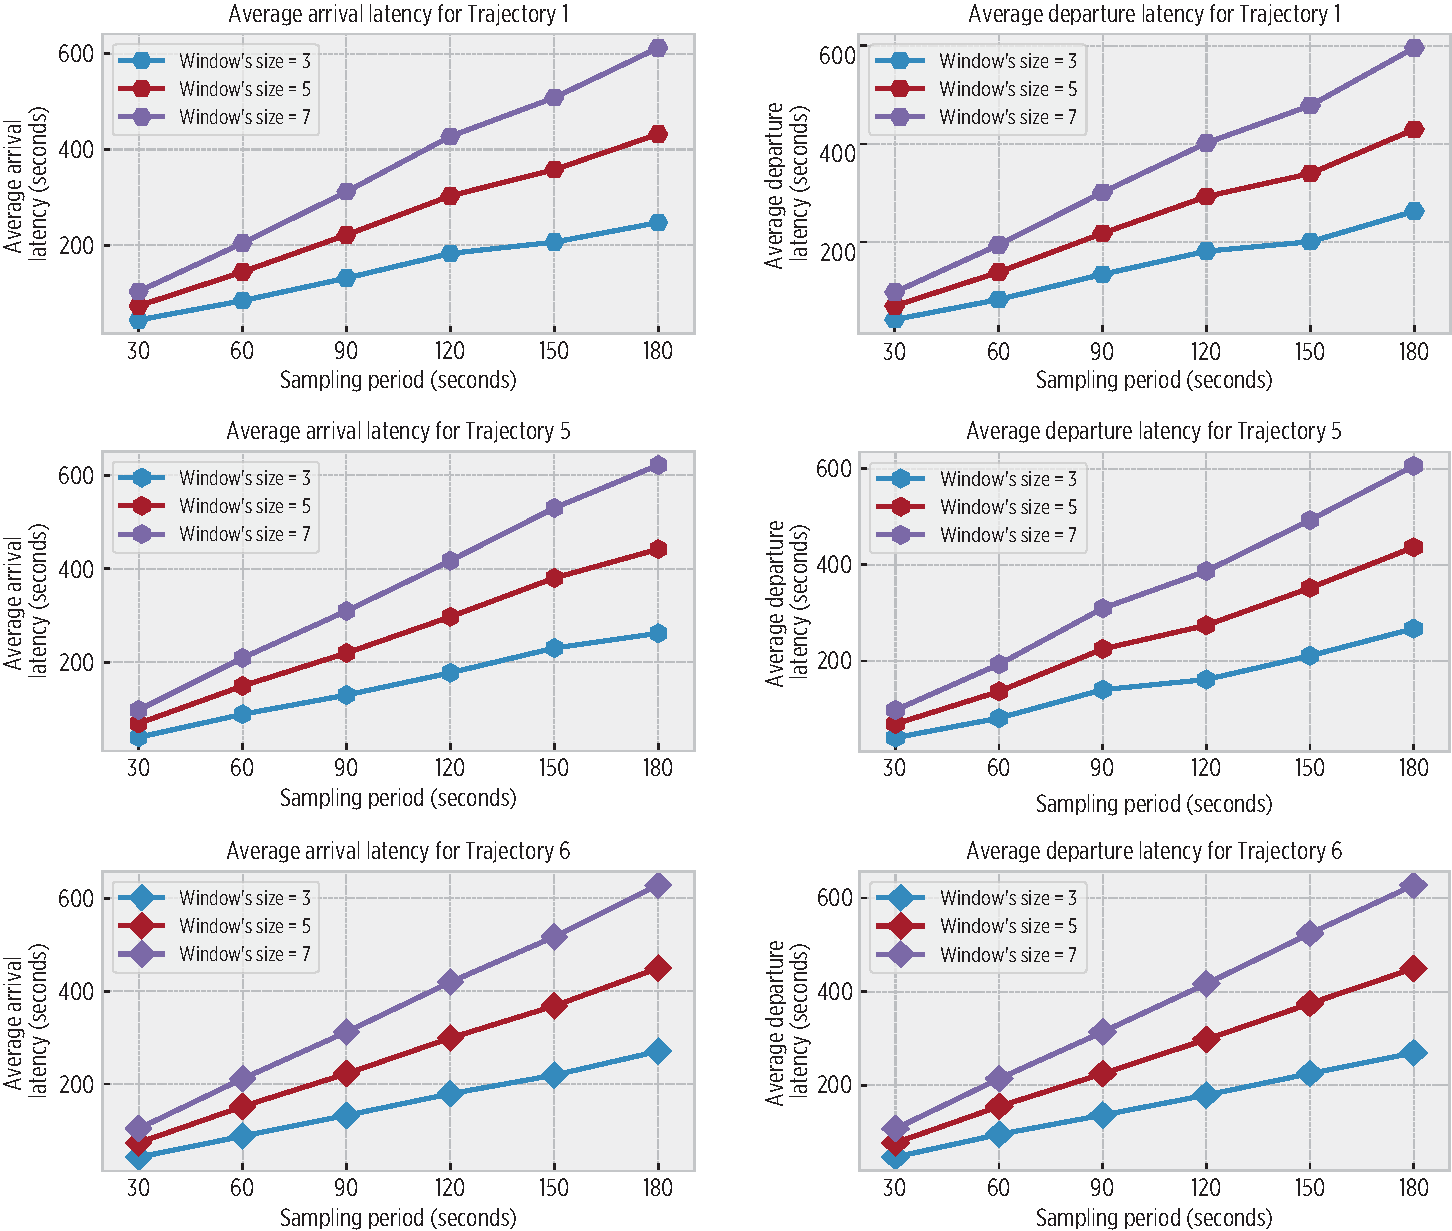
\includegraphics[width=0.75\textwidth]{vectors/experiments/exp-2/exp-2-latencies-for-slides}
  \caption{Arrival (left) and departure (right) latencies obtained by the Geofencing  module for each combination of sampling period and window length values. There is a tendency on the results as the shortest window’s sizes produce the shortest arrival latency values.}
\end{figure}
\end{frame}

\begin{frame}[noframenumbering]{Preliminary experiments}{\emph{Geofencing} module spatial-time accuracy: Results}
\vspace{-0.5cm}
\begin{figure}
  \centering
  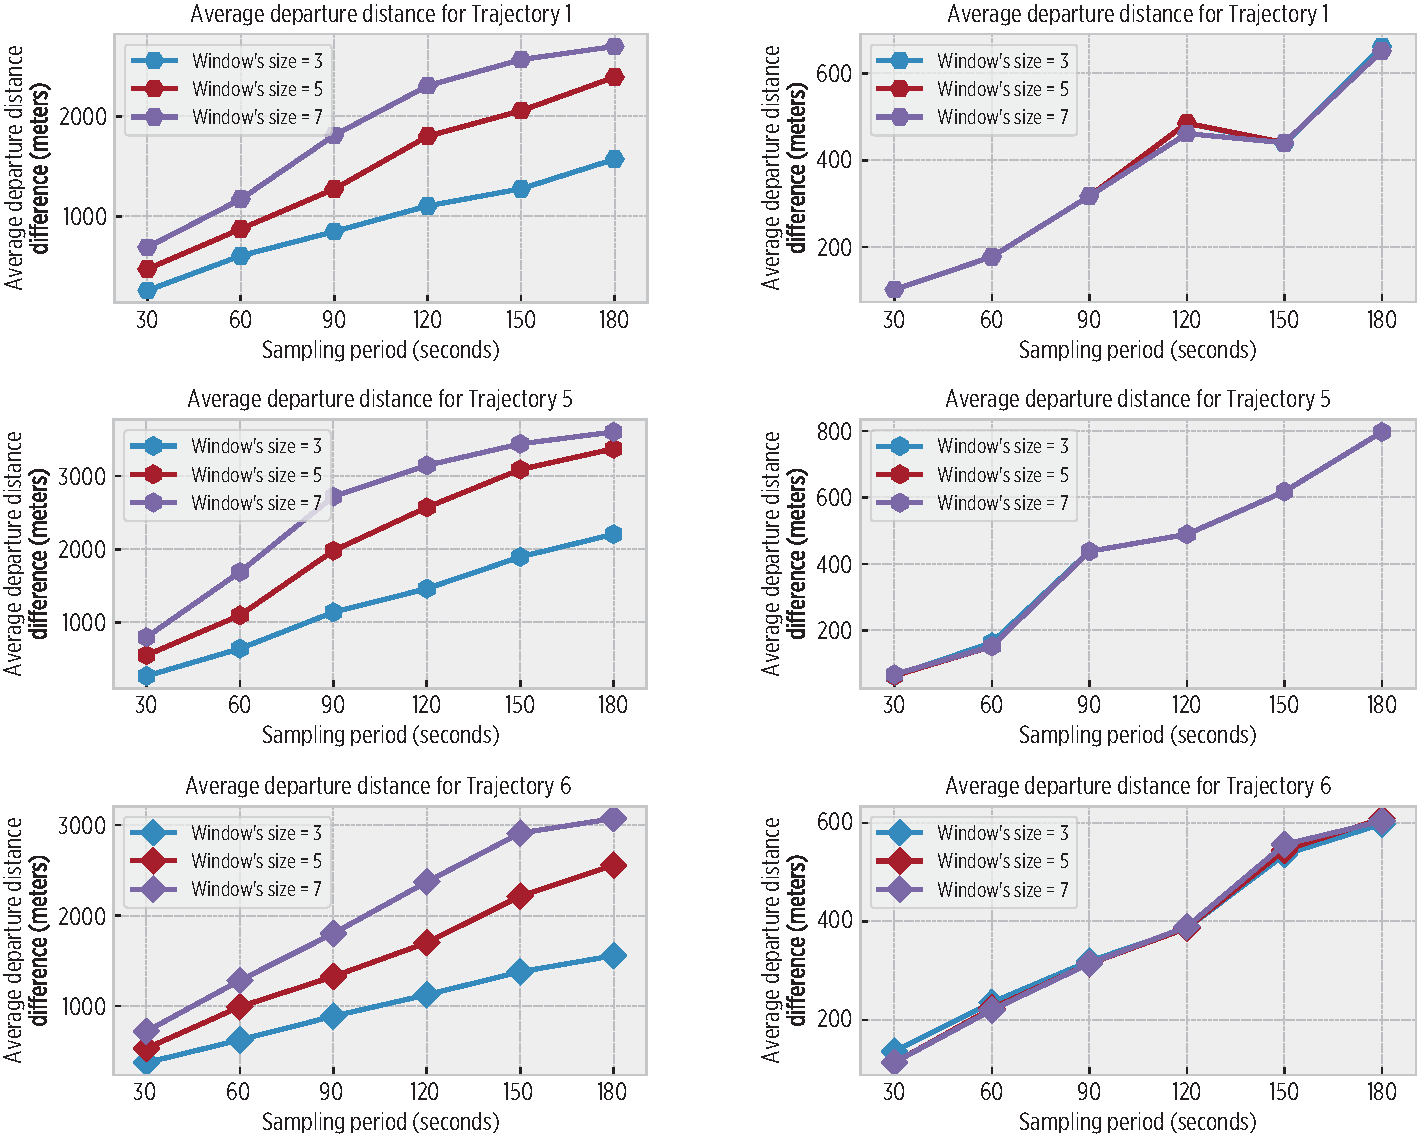
\includegraphics[width=0.77\textwidth]{vectors/experiments/exp-2/exp-2-departure-distance-for-slides}
  \caption{Departure distance difference obtained by the \emph{Geofencing} module for each combination of sampling period and window size values. On the left, the latency of the window-based geofencing is accounted, while in the right it is ignored. The high speed with which user leaves from stay points allows to identify a tendency on the results, as departures are detected earlier by shorter window sizes.}
\end{figure}
\end{frame}


\begin{frame}[noframenumbering]{Experimentation}{Holistic evaluation: Results}
\small 
\vspace{-0.5cm}
{
  \centering
  \includegraphics[width=0.7\textwidth]{vectors/experiments/exp-4/exp-4-sigmoid-header-top-row}
  \par 
}


\begin{columns}
\begin{column}[T]{0.5\textwidth}

\begin{block}{\small \textbf{Arrival distance difference}}
{
  \centering
  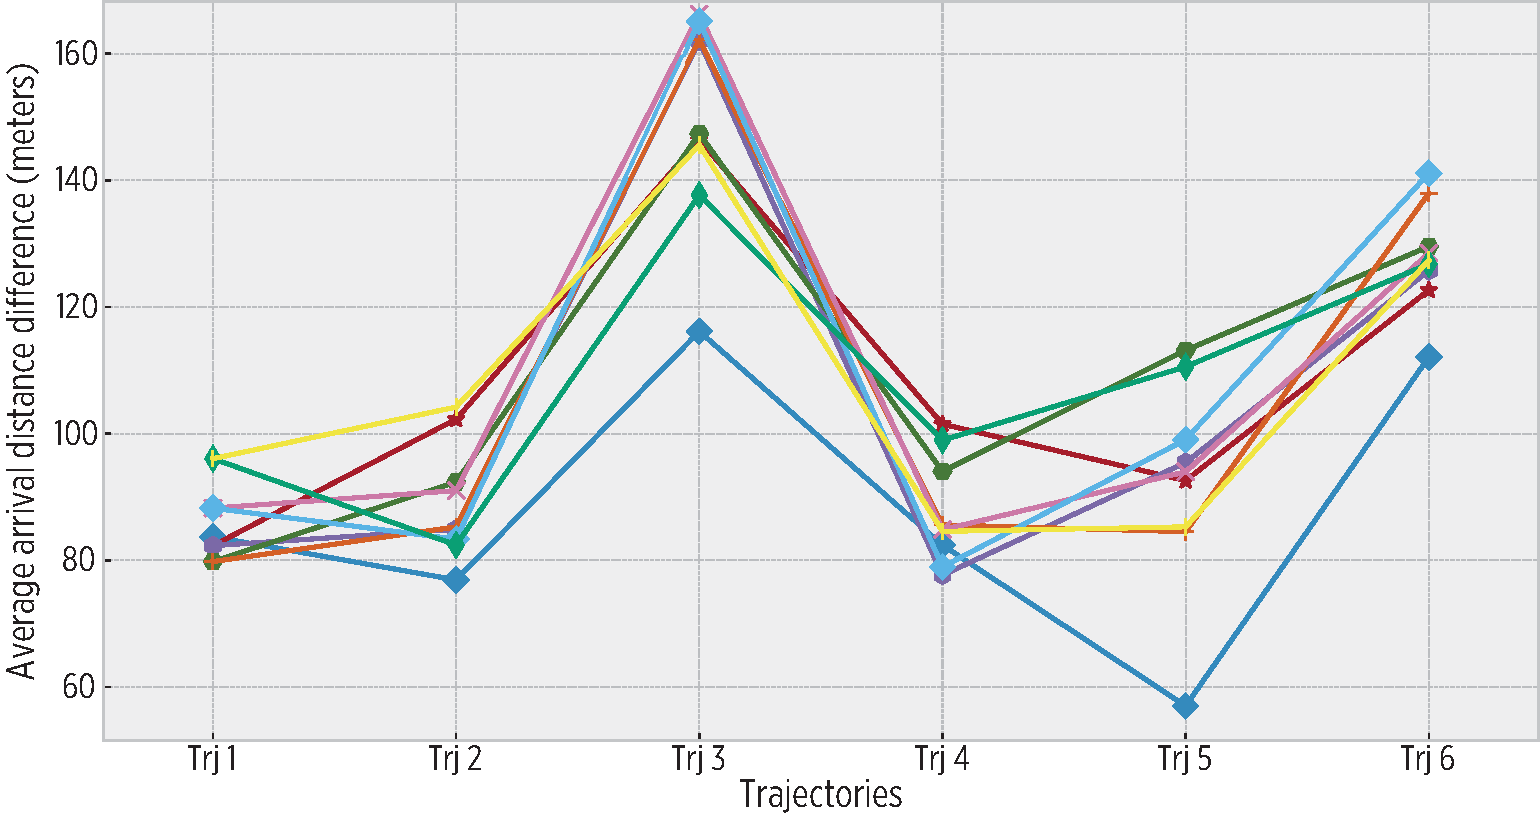
\includegraphics[width=\textwidth]{vectors/experiments/exp-4/exp-4-arrival-distance-for-slides-v2}
  \captionof{figure}{Arrival distance difference detected by the system throughout the different experimental trials. The values are shorter than for departure distance due to the decreasing speed that user describes when arriving to a stay point.}
  \par
}
\end{block}
\end{column}

\begin{column}[T]{0.5\textwidth}
\begin{block}{\small \textbf{Departure distance difference}}
{
  \centering
  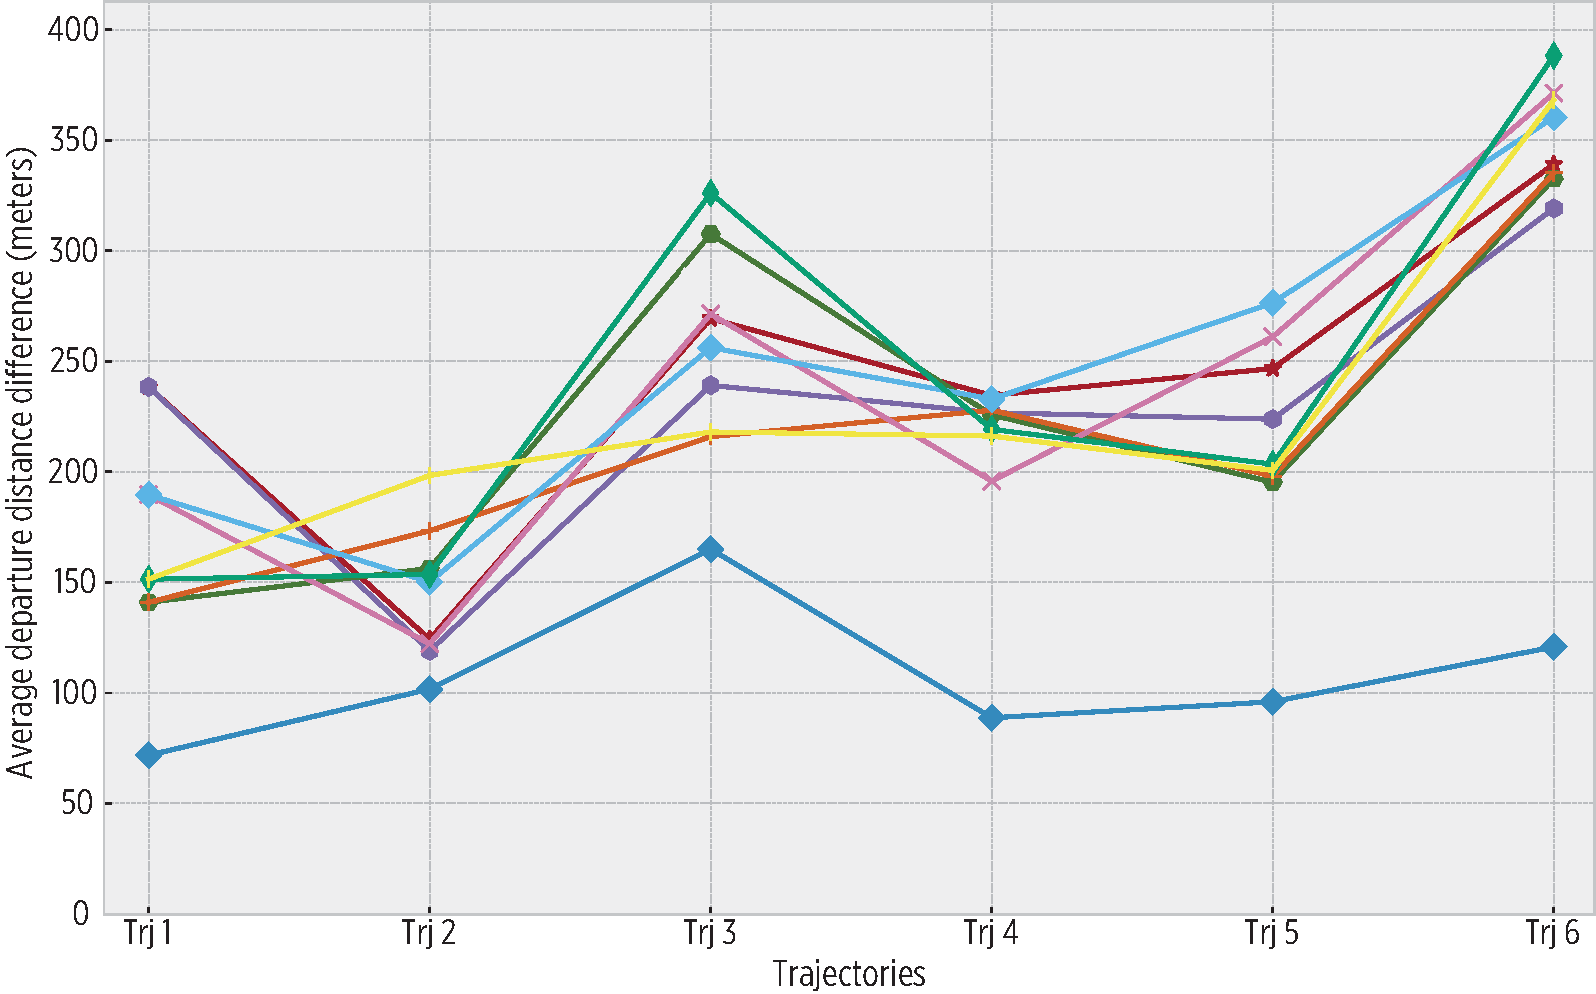
\includegraphics[width=\textwidth]{vectors/experiments/exp-4/exp-4-departure-distance-for-slides-v2}
  \captionof{figure}{Departure distance difference detected by the system throughout the different experimental trials. The larger distance differences are caused by the high speed with which user leaves the stay points (mostly using a vehicle as transportation mode).}
  \par
}
\end{block}

\end{column}
\end{columns}

\end{frame}




\begin{frame}[noframenumbering]{Preliminary experiments}{Energy saving expectations of on-device stay points detection}
\small
\vspace{-0.5cm}
\begin{columns}
\begin{column}{0.55\textwidth}
\begin{block}{\small \textbf{Description}}
\begin{itemize}
  \item This experiment explored whether a smartphone could detect stay points by itself, given its energy and computing constraints, and the energy savings of such implementation compared against typical solutions.
  \item Typical solutions implement a Mobile Cloud Computing (MCC) approach on which the smartphone only collects and offloads the processing to external servers.
\end{itemize}
\end{block}
\end{column}

\begin{column}{0.4\textwidth}
\begin{table}
\centering
\renewcommand{\arraystretch}{0.8}
\resizebox{0.95\textwidth}{!}{%
\begin{tabular}{lll}
\toprule
\multirow{2}{*}{\textbf{Stay Points Detector}} & \textbf{Time threshold} ($\delta_{time}$): & $45~min$ \\
\cmidrule[0.25pt]{2-3}
 & \textbf{Distance threshold} ($\delta_{distance}$): & $500~m$ \\

\cmidrule[0.25pt]{1-3}
\textbf{Sampling periods}: & \multicolumn{2}{l}{30, 60, 90, 120, 150 seconds} \\
\bottomrule
\end{tabular}
}
\caption{Input parameters for the energy saving expectations of on-device stay points detection experiment.}
\end{table}
\end{column}
\end{columns}

\begin{block}{\small \textbf{Results}}
%\begin{table}
\vspace{1em}
{\centering
\resizebox{0.9\textwidth}{!}{%
\renewcommand{\arraystretch}{0.9}
\begin{tabular}{@{}cccccccc@{}}
\toprule
\textbf{\begin{tabular}[c]{@{}c@{}}Sampling\\period (seconds)\end{tabular}}  &
\textbf{\begin{tabular}[c]{@{}c@{}}Processing\\ strategy\end{tabular}}
& \textbf{\begin{tabular}[c]{@{}c@{}}Location update \\ requests\end{tabular}}
& \textbf{\begin{tabular}[c]{@{}c@{}}GPS-on time\\ (minutes)\end{tabular}}
& \textbf{\begin{tabular}[c]{@{}c@{}}Average acquisition \\  time per fix (seconds)\end{tabular}}
& \textbf{\begin{tabular}[c]{@{}c@{}}Total experiment \\ time (minutes)\end{tabular}}
& \textbf{\begin{tabular}[c]{@{}c@{}}Data sent\\ (bytes)\end{tabular}}
& \textbf{\begin{tabular}[c]{@{}c@{}}Data received\\ (bytes)\end{tabular}} \\ \midrule

\multirow{2}{*}{30}  & On-device   &  12,365 & 1,614 & 7.83  & 7,790 & - & - \\
                          & MCC &  9,324 &   770 & 4.95  & 5,402 & 1,084,901 & 18,796 \\
\cmidrule(l){2-8}
\multirow{2}{*}{60}  & On-device    & 10,851 & 1,219 & 6.74 & 12,028 & - & - \\
                          & MCC &  7,210 &   764 & 6.35 &  7,907 & 838,640 & 14,696 \\
\cmidrule(l){2-8}
\multirow{2}{*}{90}  & On-device    & 7,935 & 1,178 & 8.90 & 13,075 & - & - \\
                          & MCC & 5,626 &   546 & 5.82 &  8,946 & 653,833 & 12,223 \\
\cmidrule(l){2-8}
\multirow{2}{*}{120} & On-device    & 5,246 & 809 & 9.25 & 11,289 & - & - \\
                          & MCC & 4,333 & 387 & 5.35 &  8,931 & 504,012 & 8,838 \\
\cmidrule(l){2-8}
\multirow{2}{*}{150} & On-device    & 5,635 & 933 & 9.93 & 14,998 & - & - \\
                          & MCC & 4,566 & 452 & 5.93 & 11,619 & 530,764 & 10,309 \\
\bottomrule
\end{tabular}%
}
\captionof{table}{Summary of experimental results of on-device vs. MCC approach comparison.}
%\caption{Summary of experimental results of on-device vs. MCC approach comparison.}
%\label{tab:on-device-mcc-comparison}
%\end{table}
\par }
\end{block}
\end{frame}


\begin{frame}[noframenumbering]{Experimentation}{Energy saving expectations of on-device stay points detection}
\small
% \vspace{-0.5cm}
\begin{columns}
\begin{column}{0.55\textwidth}
\begin{block}{\small \textbf{Description}}
\begin{itemize}
  \item This experiment explored whether a smartphone could detect stay points by itself, and the energy savings of such implementation with respect of typical Mobile Cloud Computing (MCC) based solutions.
  % \item Typical solutions implement a Mobile Cloud Computing (MCC) approach on which the smartphone only collects and offloads the processing to external servers.
\end{itemize}
\end{block}
\end{column}

\begin{column}{0.4\textwidth}
\begin{table}
\centering
\renewcommand{\arraystretch}{0.8}
\resizebox{0.95\textwidth}{!}{%
\begin{tabular}{lll}
\toprule
\multirow{2}{*}{\textbf{Stay Points Detector}} & \textbf{Time threshold} ($\delta_{time}$): & $45~min$ \\
\cmidrule[0.25pt]{2-3}
 & \textbf{Distance threshold} ($\delta_{distance}$): & $500~m$ \\

\cmidrule[0.25pt]{1-3}
\textbf{Sampling periods}: & \multicolumn{2}{l}{30, 60, 90, 120, 150 seconds} \\
\bottomrule
\end{tabular}
}
\caption{Input parameters for the energy saving expectations of on-device stay points detection experiment.}
\label{tab:exp-energy-performance-input-parameters}
\end{table}
\end{column}
\end{columns}

\begin{figure}
  \centering
  \includegraphics[width=\columnwidth]{vectors/local-poi-article/plot-energy-performance-r2-for-slides}
  \caption{Energy performance comparison of on-device vs. MCC sample apps using different GPS sampling periods. Each of the on-device trials last longer than its corresponding remote implementation.}
\end{figure}

\end{frame}



\begin{frame}[noframenumbering]{Experimentation}{Comparison with other solutions}
\begin{table}[]
\centering
\small
\renewcommand{\arraystretch}{1.2}
\begin{tabular}{@{}p{1cm}p{1.8cm}p{1.6cm}p{1.4cm}p{1cm}p{1cm}@{}}
\toprule
\textbf{Work} &
\textbf{Purpose} &
\textbf{Mobility type} &
\textbf{Involved sensors} &
\textbf{Trajectory tracking} &
\textbf{Place learning} \\ 
\midrule

\textbf{SenseLess} &
Location tracking &
Walking, static &
Accelerometer, GPS &
Yes &
No \\

\cmidrule[0.25pt]{1-6}
\textbf{SmartDC} &
Place tracking &
Not specified &
Cellular id, Wi-Fi, GPS&
No &
Yes \\

\cmidrule[0.25pt]{1-6}
Proposed system &
Location and place tracking &
Static, walking, biking, vehicle &
Accelerometer, GPS &
Yes &
Yes \\

\bottomrule
\end{tabular}%

\caption{Features comparison of proposed system and representative existing solutions.}
\end{table}
\end{frame}


\begin{frame}[noframenumbering]{Preliminary results}{Comparison with other solutions}
\begin{table}[]
\centering
\small
\tabcolsep=0.12cm
\renewcommand{\arraystretch}{1.2}
\begin{tabular}{@{}p{1cm}p{2cm}p{2.5cm}p{2cm}p{3cm}@{}}
\toprule
\textbf{Work} &
\textbf{Place learning technique} &
\textbf{Sampling adaptation technique} &
\textbf{Energy metric} &
\textbf{Energy result} \\ 
\midrule

\textbf{SenseLess} &
None &
Simple Decision Rule (static, motion) &
Energy profiling of sensors &
41\% consumption (of a fixed $10 s$ GPS sampling) \\

\cmidrule[0.25pt]{1-5}
\textbf{SmartDC} &
Wi-Fi fingerprinting &
Markov Decision Process (time series mobility predictor and energy budget). &
Energy profiling of sensors &
81\% less than a periodic sensing scheme.\\

\cmidrule[0.25pt]{1-5}
Proposed system &
GPS Stream-based SPs detection, Geofencing, time-aware visits analysis. &
Cognitive controller (sigmoid sampling) &
Battery lifetime, amount of location updates &
{
Simulation: 14\%, 42\% location updates (of fixed $10 s$, $30 s$ GPS sampling).

On device deployment: 53 hours battery life increase, 77\% location updates (of a fixed $30 s$ GPS sampling), 
}\\

\bottomrule
\end{tabular}%

\caption{Results comparison of proposed system and representative existing solutions.}
\end{table}
\end{frame}



% \begin{frame}[noframenumbering]{Detailed schedule}
% \begin{table}[]
% \centering
% \resizebox{0.95\textwidth}{!}{%
% \begin{tabular}{clccccccc}
%    &                                                                               & 2014 & \multicolumn{3}{c}{2015} & \multicolumn{3}{c}{2016}  \\
%    \cline{3-9}
% \multicolumn{2}{l}{\small{Work: \markdone~Done, \markonprogress~In progress, \markoff~To be done}} & 3rd & 1st & 2nd & 3rd & 1st & 2nd & 3rd \\
%    \toprule
% \multicolumn{2}{c}{\textsc{Step I}}                                                &  &  &  &  &  &  &  \\
% 1  & State-of-art reading                                                          & \markdone & \markdone &  &  &  &  &  \\
% 2  & State-of-art works categorization                                             &  & \markdone & \markdone  &  &  &  &  \\
% 3  & Documentation of information found (committee request)                        &  &  & \markdone &  &  &  &  \vspace{1em}\\

% \multicolumn{2}{c}{\textsc{Step II}}                                               &  &  &  &  &  &  &  \\
% 4  & \makecell[l]{Development of a mobile app for accelerometer and location \\data collection}    &  &  & \markdone & \markdone  &  &  &  \\
% 5  & Analysis of data                                                              &  &  &  & \markdone  &  &  &  \\
% 6  & Formal definition of mobility pattern                                         &  &  &  & \markdone &  &  &  \\
% 7  & Selection of mobility patterns                                                &  &  &  & \markdone & \markdone &  &  \vspace{1em}\\

% \multicolumn{2}{c}{\textsc{Step III}}                                              &  &  &  &  &  &  &  \\
% 8  & Research on classification algorithms for mobility patterns                   &  &  &  & \markdone & \markdone &  &  \\
% 9  & Definition of metrics for evaluating algorithms                               &  &  &  &  & \markdone &  &  \\
% 10 & Implementation of algorithms in mobile platform                               &  &  &  &  & \markdone & \markdone  &  \\
% 11 & Selection of best algorithms according to metrics                             &  &  &  &  &  & \markdone &  \vspace{1em}\\

% \multicolumn{2}{c}{\textsc{Step IV}}                                               &  &  &  &  &  &  &  \\
% 12 & Definition and modeling of parameters needed by the \emph{Mobility Events Detector}                       &  &  &  & \markdone & \markdone & \markdone & \markdone \\
% 13 & Development of the \emph{Mobility Events Detector}.  &  &  &  & \markdone & \markdone & \markdone & \markdone \\
% \bottomrule
% \end{tabular}%
% }
% \caption{Schedule of activities (each column represents a four months period)}
% \end{table}
% \end{frame}

% \begin{frame}[noframenumbering]{Detailed schedule}
% \begin{table}[]
% \centering
% \resizebox{0.95\textwidth}{!}{%
% \begin{tabular}{clccccccc}
%    &                                                                               & \multicolumn{3}{c}{2016} & \multicolumn{3}{c}{2017} & 2018 \\
%    \cline{3-9}
% \multicolumn{2}{l}{\small{Work: \markdone~Done, \markonprogress~In progress, \markoff~To be done}}   & 1st & 2nd & 3rd & 1st & 2nd & 3rd & 1st \\
%    \toprule
% \multicolumn{2}{c}{\textsc{Step V}}                                                &  &  &  &  &  &  & \\
% 14  & Formal definition of policy                                                  &  &  & \markdone &  &  &  & \\
% 15  & \makecell[l]{Research and evaluation of techniques for\\generation and adaption of policies}&  &  & \markdone & \markdone  &  &  & \\
% 16  & Design and execution of experiments applied to use cases                     &  &  & \markdone & \markdone  &  &  & \\
% 17  & Selection of policies                                                        &  &  &  & \markdone  &  &  & \vspace{1em} \\

% \multicolumn{2}{c}{\textsc{Step VI}}                                               &  &  &  &  &  &  & \\
% 18  & Definition and modeling of Cognitive Controller parameters                                    &  &  &  &  & \markdone  &  & \\
% 19  & Development of the Cognitive controller                                                          &  &  &  &  & \markdone  &  & \vspace{1em} \\

% \multicolumn{2}{c}{\textsc{Step VII}}                                               &  &  &  &  &  &  & \\
% 20  & Analysis of components into software abstractions                             &  &  &  &  & \markdone  &  & \\
% 21  & Research on Android API for specialized components                            &  &  &  &  & \markdone  &  & \\
% 22  & Development of middleware                                                     &  &  &  &  & \markdone  &  & \vspace{1em}\\

% \multicolumn{2}{c}{\textsc{Step VIII}}                                              &  &  &  &  &  &  & \\
% 23  & \makecell[l]{Definition of experiments aimed at accuracy\\and energy consumption metrics}    &  &  &  &  &  & \markdone & \\
% 24  & Development of experimental sample mobile apps                                &  &  &  &  &  & \markonprogress & \\
% 25  & Experiments execution                                                         &  &  &  &  &  & \markonprogress & \markoff  \\
% 26  & Final results analysis                                                              &  &  &  &  &  &  & \markoff \\
% \bottomrule
% \end{tabular}%
% }
% \caption{Schedule of activities (each column represents a four months period)}
% \end{table}
% \end{frame}

% \begin{frame}[noframenumbering]{Detailed schedule}
% \begin{table}
% \centering
% \resizebox{\textwidth}{!}{%
% \begin{tabular}{clcccccccccccc}
%    &                                                                               & 2014 & \multicolumn{3}{c}{2015} & \multicolumn{3}{c}{2016} & \multicolumn{3}{c}{2017} & \multicolumn{2}{c}{2018} \\
%    \cline{3-14}
%  \multicolumn{2}{l}{\small{Work: \markdone~Done, \markonprogress~In progress, \markoff~To be done}} & 3rd & 1st & 2nd & 3rd & 1st & 2nd & 3rd & 1st & 2nd & 3rd & 1st & 2nd\\
%    \toprule
% \multicolumn{2}{c}{\textsc{Required tasks}}                                        &  &  &  &  &  &  &  &  &  &  &  & \\
% A   & Related courses                                                              & \markdone  & \markdone  & \markdone &  &  &  &  &  &  &  &  & \\
% B   & Research articles submission                                                 &  &  &  & \markdone &  & \markdone &  &  &  &  & \markonprogress & \\
% C   & Predoctoral exam preparation                                                 &  &  &  &  &  &  &  &  & \markdone &  &  & \\
% D   & Thesis writing                                                               & \markdone  &  &  & \markdone &  &  & \markdone &  &  & \markonprogress & \markoff & \markoff \\

% \bottomrule
% \end{tabular}%
% }
% \caption{Schedule of required activities}
% \end{table}
% \end{frame}


% \begin{frame}[noframenumbering]{Layered perceptual memory}{Short and long-term memory information}
% \vspace{-0.25cm}
% \small
% \begin{block}{\small \textbf{Layered perceptual memory}}
% \begin{itemize}
%     \item Short-term memory information: current (observed) mobility status.
%     \item Long-term memory information: the Expanded Spatial-Time model (STM).
% \end{itemize}
% \end{block}

% \begin{block}{\small \textbf{Expanded Spatial-Time model}}
% \begin{itemize}
%   \item The highest level of mobility information held by the system.
% \end{itemize}
% {
%   \centering
%   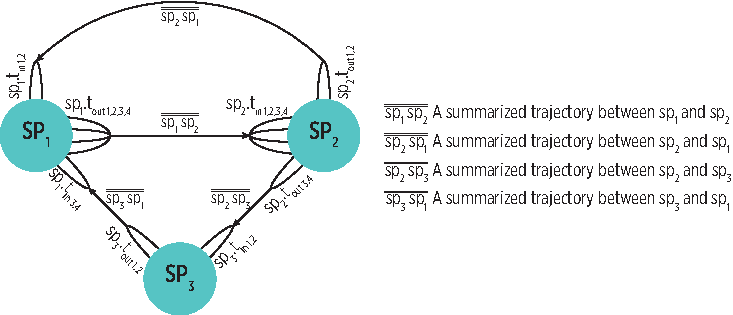
\includegraphics[width=0.75\textwidth]{vectors/stm-slides}
%   \captionof{figure}{A conceptual representation of the STM's structure.}
% \par }
% \end{block}
% \end{frame}

% \begin{frame}[noframenumbering]{Layered perceptual memory}{Expanded Spatial-Time model (STM)}
% \small
% \begin{block}{\small \textbf{Generation of the STM}}
% \begin{itemize}
%     \item Incrementally built with the coarse-grain mobility events detected by the \emph{Mobility Events Detector}.
% \end{itemize}
% {
%   \centering
%   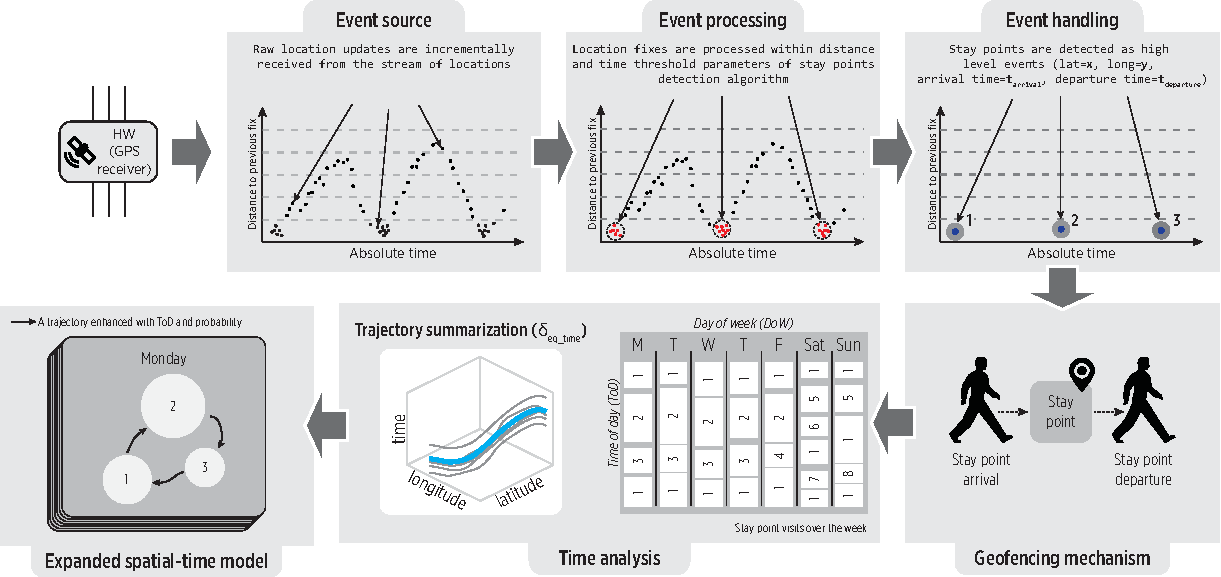
\includegraphics[width=\textwidth]{vectors/event-driven-memory-generation-for-slides}
%   \captionof{figure}{A conceptual representation of the steps for generating the STM from raw sensors data.}
%   \par
% }
% \end{block}
% \end{frame}


% \begin{frame}[noframenumbering]{Cognitive controller (CC)}{Description}
% \small
% \vspace{-0.5cm}
% \begin{columns}
% \begin{column}[T]{0.5\textwidth}
% \begin{block}{\small \textbf{Goals}}
%   \begin{itemize}
%       \item To reduce the energy consumption of location tracking by relying on PRM's estimations.
%       \item To reduce the system uncertainty about current user mobility.
%   \end{itemize}
% \end{block}
% \end{column}

% \begin{column}[T]{0.5\textwidth}
% \begin{block}{\small \textbf{Possible cognitive actions}}
%   \begin{itemize}
%     \item \textbf{Exploitation policies}: When system uncertainty is low for saving energy purposes.
%     \item \textbf{Exploration policies}: When system uncertainty is high for recovering for accuracy loss.
%   \end{itemize}
% \end{block}
% \end{column}
% \end{columns}

% \begin{figure}
%   \centering
%   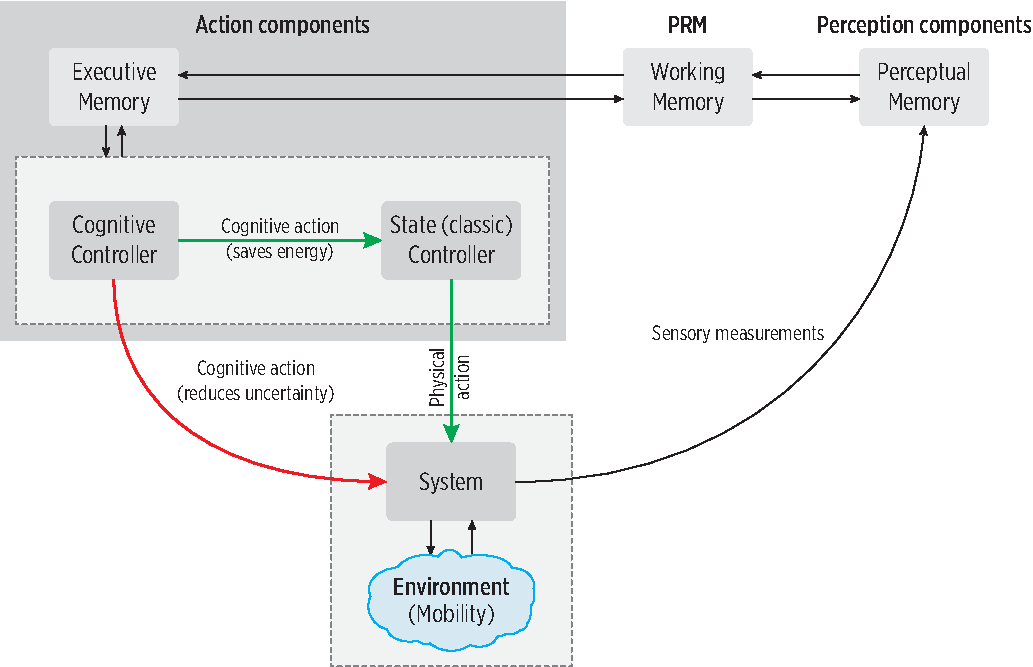
\includegraphics[width=0.65\textwidth]{vectors/cognitive-controller-architecture}
%   \caption{A generic cognitive controller architecture}
% \end{figure}
% \end{frame}

% \begin{frame}[noframenumbering]{Cognitive controller}{Policies tailored for user mobility}
% \small
% \begin{block}{\small \textbf{Stay point mode}}
%   \begin{itemize}
%       \item A sampling based on the sigmoid function $sig(x) = \frac{1}{1+e^{-\alpha x}}$ as a model for the mobility phase transitions.
%       \item Higher sampling rate on arrival and departure, when the user is more likely to move, and slower at the middle of a visit.
%   \end{itemize}
% \end{block}

% \begin{columns}
% \begin{column}{0.45\textwidth}
% \begin{figure}
%   \centering
%   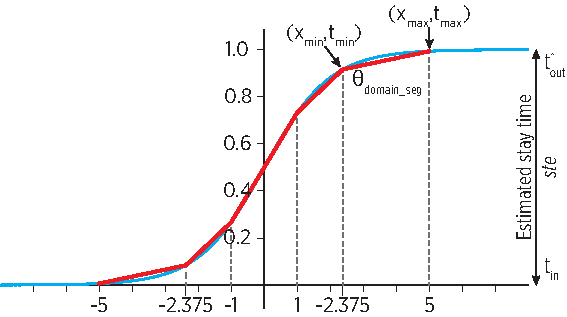
\includegraphics[width=0.99\linewidth]{vectors/sigmoid-segmentation-for-slides}
%   \caption{Approximation of the sigmoid through straight segments.}
% \end{figure}
% \end{column}

% \begin{column}{0.55\textwidth}
% \begin{figure}
%   \centering
%   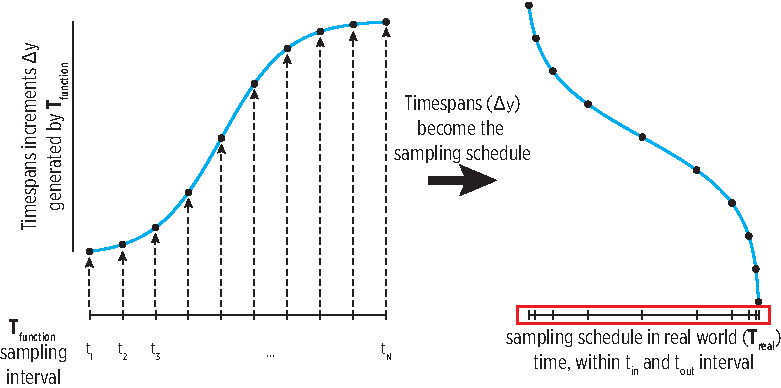
\includegraphics[width=0.99\linewidth]{vectors/sigmoid-driven-sampling-policy-for-slides}
%   \caption{A snapshot of the process for producing a sigmoid sampling.}
% \end{figure}
% \end{column}
% \end{columns}
% \end{frame}

% \begin{frame}[noframenumbering]{Preliminary experimentation}{\emph{Stay Points Detector} module spatial-time accuracy}
% \small

% \begin{columns}
% \begin{column}[T]{0.55\textwidth}

% \begin{block}{\small \textbf{Description}}
% \begin{itemize}
%   \item This experiment evaluates the spatial-time accuracy of the \emph{Stay Points Detector} module under different GPS sampling rates in terms of centroid distances and latencies.
% \end{itemize}
% \end{block}

% \end{column}
% \begin{column}[T]{0.45\textwidth}
% \begin{table}
% \centering
% \renewcommand{\arraystretch}{0.6}
% \resizebox{0.9\textwidth}{!}{%
% \begin{tabular}{lll}
% \toprule
% \multirow{2}{*}{\textbf{Stay Points Detector}} & \textbf{Time threshold} ($\delta_{time}$): & $45~min$ \\
% \cmidrule[0.25pt]{2-3}
%  & \textbf{Distance threshold} ($\delta_{distance}$): & $500~m$ \\

% \cmidrule[0.25pt]{1-3}
% \textbf{Sampling periods}: & \multicolumn{2}{l}{30, 60, 90, 120, 150, 180 seconds.} \\

% \cmidrule[0.25pt]{1-3}
% \textbf{Trajectories}: & \multicolumn{2}{l}{All ground truth trajectories.} \\
% \bottomrule
% \end{tabular}
% }
% \caption{Input parameters for the spatial-time accuracy of stay points experiment.}
% \end{table}
% \end{column}
% \end{columns}

% \vspace{-0.5cm}
% \begin{block}{\small \textbf{Results}}
% \begin{columns}
% \begin{column}{0.65\textwidth}
% \begin{figure}
%   \centering
%   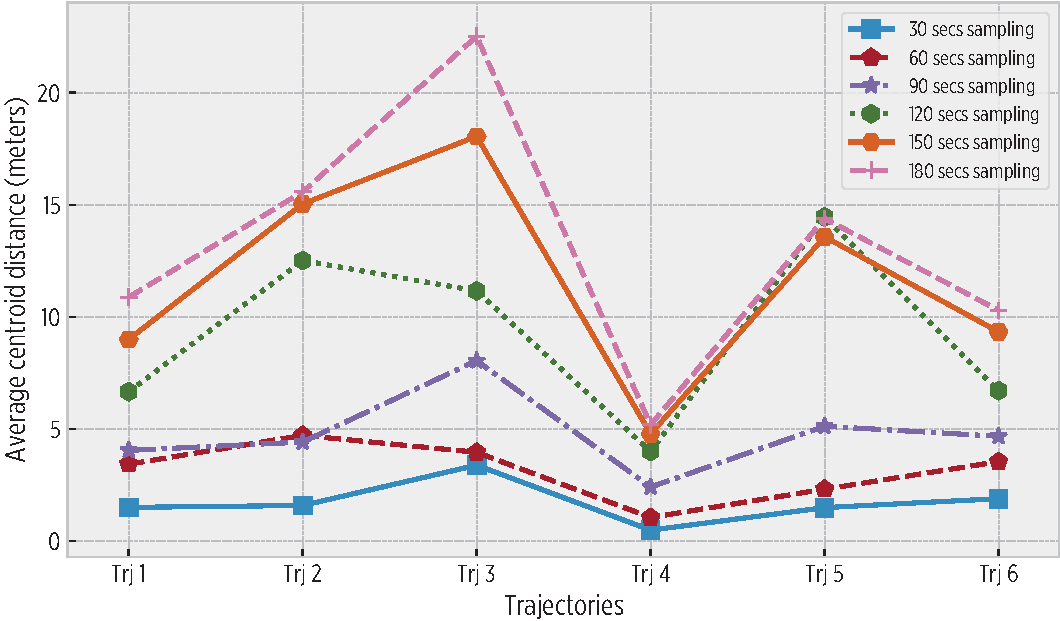
\includegraphics[width=0.99\textwidth]{vectors/exp-1-centroid-distance}
% \end{figure}
% \end{column}
% \begin{column}{0.3\textwidth}
% \captionof{figure}{The impact of different sampling periods on the centroid distance of identified stay points in each trajectory. A maximum centroid distance of $22.52~m$ is identified when employing the 180 seconds sampling period.}
% \end{column}
% \end{columns}

% \end{block}
% \end{frame}


% \begin{frame}[noframenumbering]{Preliminary experimentation}{\emph{Geofencing} module spatial-time accuracy: Results}
% \vspace{-0.5cm}
% \begin{figure}
%   \centering
%   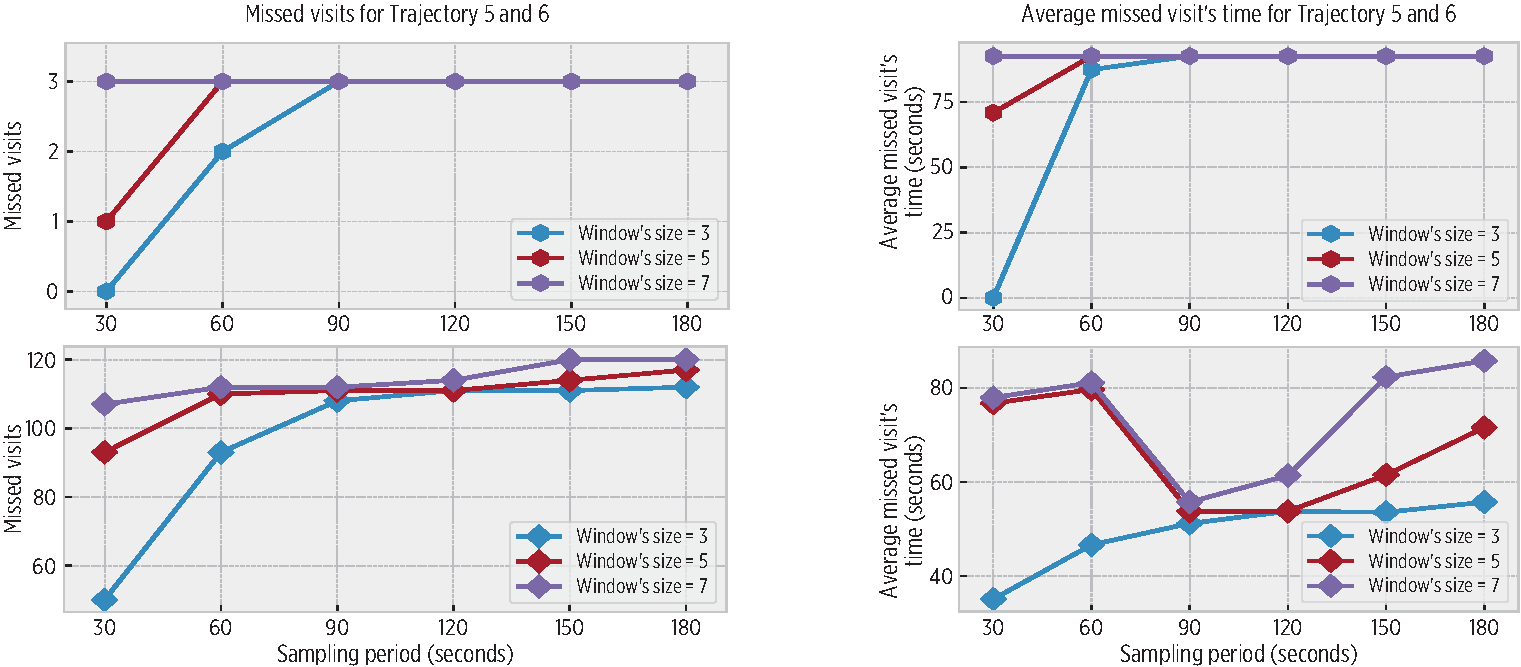
\includegraphics[width=0.78\textwidth]{vectors/exp-2-visits-for-slides}
%   \caption{Visits missed by the \emph{Geofencing} module for each combination of sampling period and window size values. The largest amount is obtained for the \emph{Trajectory 6}, given its length (more than 30 days). Nevertheless, they do not account for a considerable time in overall trajectories.}
% \end{figure}
% \end{frame}


% \begin{frame}[noframenumbering]{Preliminary experimentation}{Holistic evaluation: Results}
% \small 
% \vspace{-0.5cm}
% {
%   \centering
%   \includegraphics[width=0.7\textwidth]{vectors/exp-4-sigmoid-header-top-row}
%   \par 
% }

% \begin{columns}
% \begin{column}[T]{0.48\textwidth}
% \begin{block}{\small \textbf{Arrival latency}}
% {
%   \centering
%   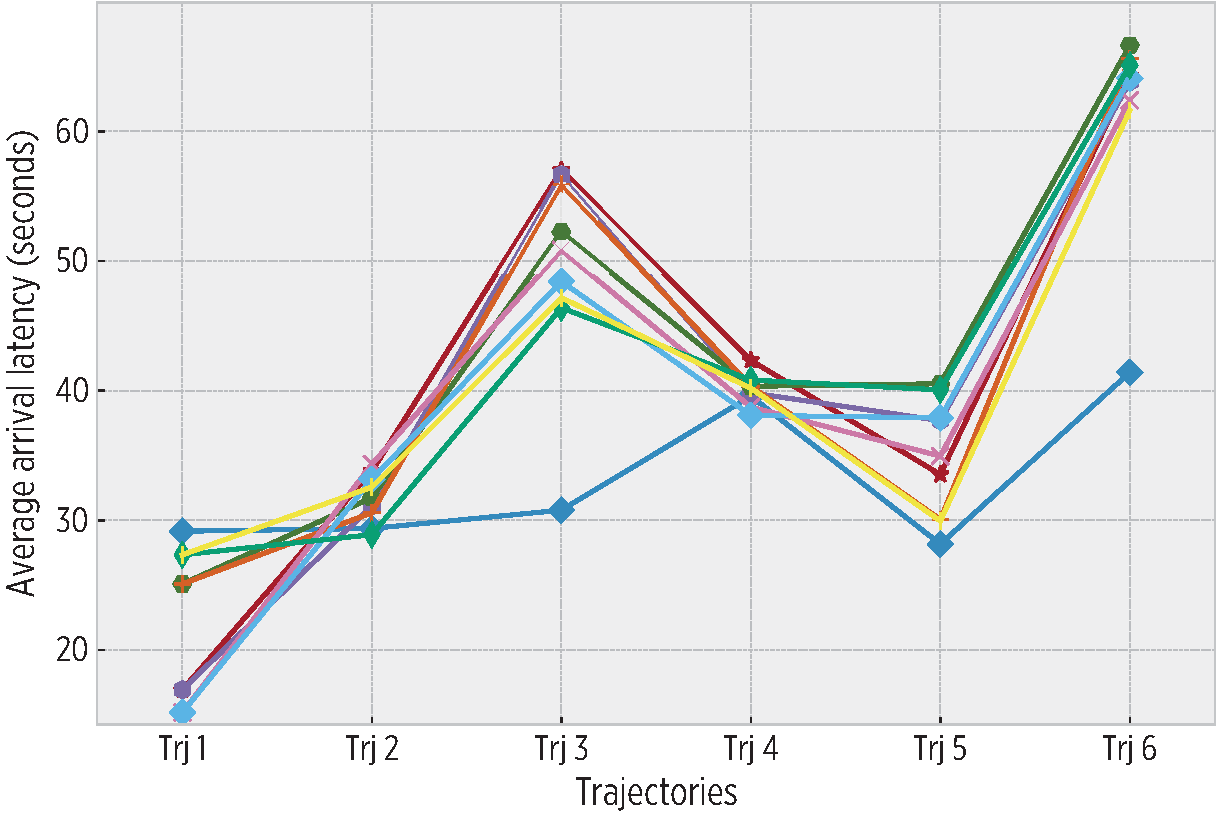
\includegraphics[width=\textwidth]{vectors/exp-4-arrival-latency-for-slides-v2}
%   \captionof{figure}{Arrival latency observed by the platform in experimental trials. The largest average value is below 65 seconds, explained by the fact that 2 location updates must be collected by the \emph{Geofencing} module before identifying an arrival event.}
%   \par 
% }
% \end{block}
% \end{column}

% \begin{column}[T]{0.52\textwidth}
% \begin{block}{\small \textbf{Departure latency}}
% {
%   \centering
%   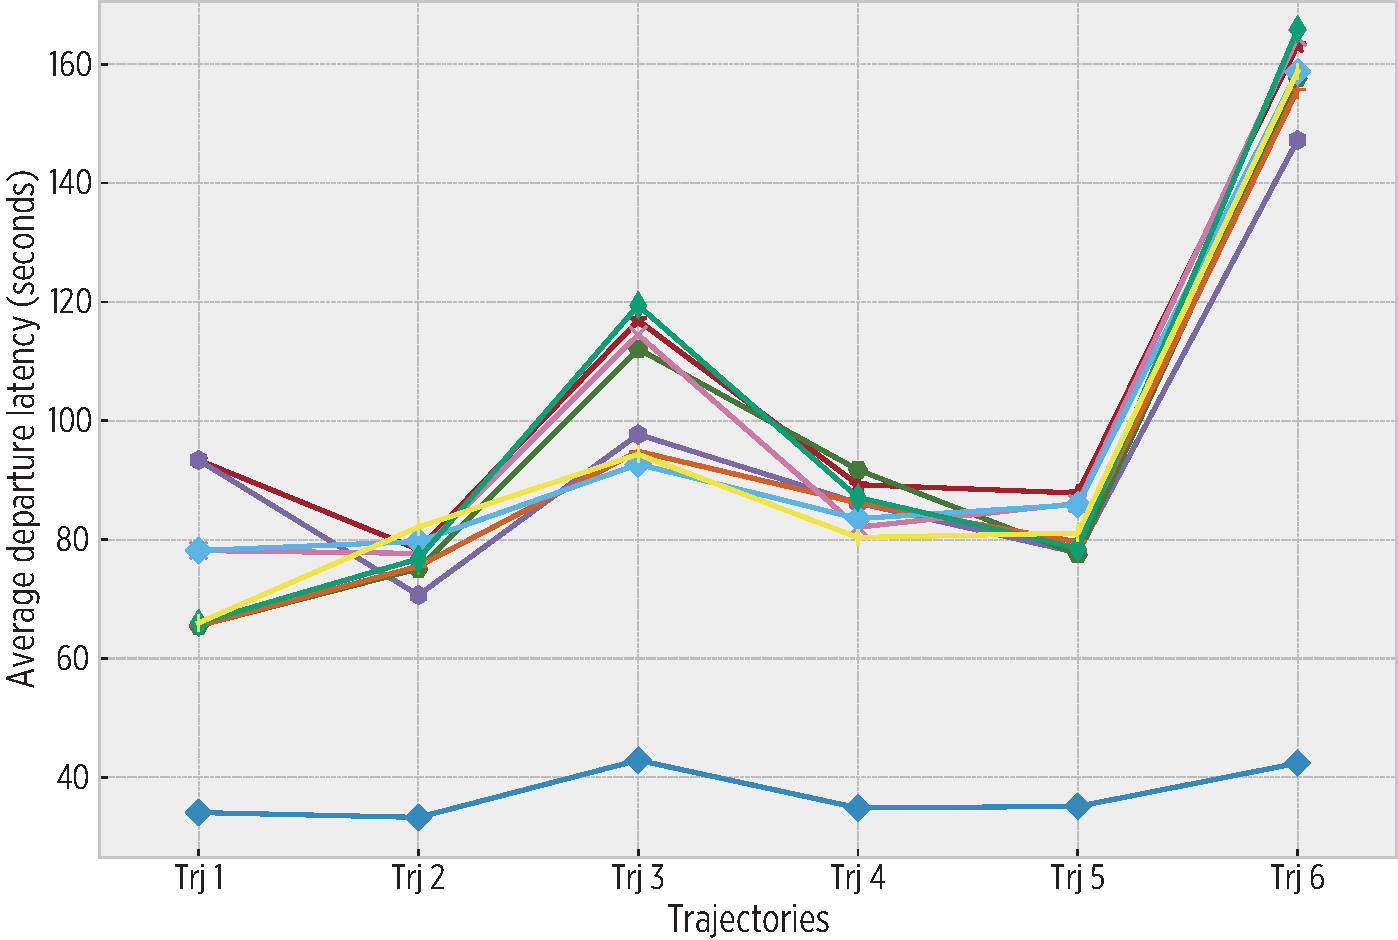
\includegraphics[width=\textwidth]{vectors/exp-4-departure-latency-for-slides-v2}
%   \captionof{figure}{Departure latency observed by the platform across performed experimental trials. The latencies are within 65 and 165 seconds, which is aligned with the different values specified to the CC for its sigmoid-driven sampling.}
%   \par
% }
% \end{block}
% \end{column}
% \end{columns}
% \end{frame}

% \begin{frame}[noframenumbering]{Preliminary experimentation}{Holistic evaluation: Results}
% \small
% \vspace{-0.5cm}
% {
%   \centering
%   \includegraphics[width=0.7\textwidth]{vectors/exp-4-sigmoid-header-top-row}
%   \par 
% }

% \begin{columns}
% \begin{column}[T]{0.5\textwidth}

% \begin{block}{\small \textbf{Trajectory distance difference}}
% {
%   \centering
%   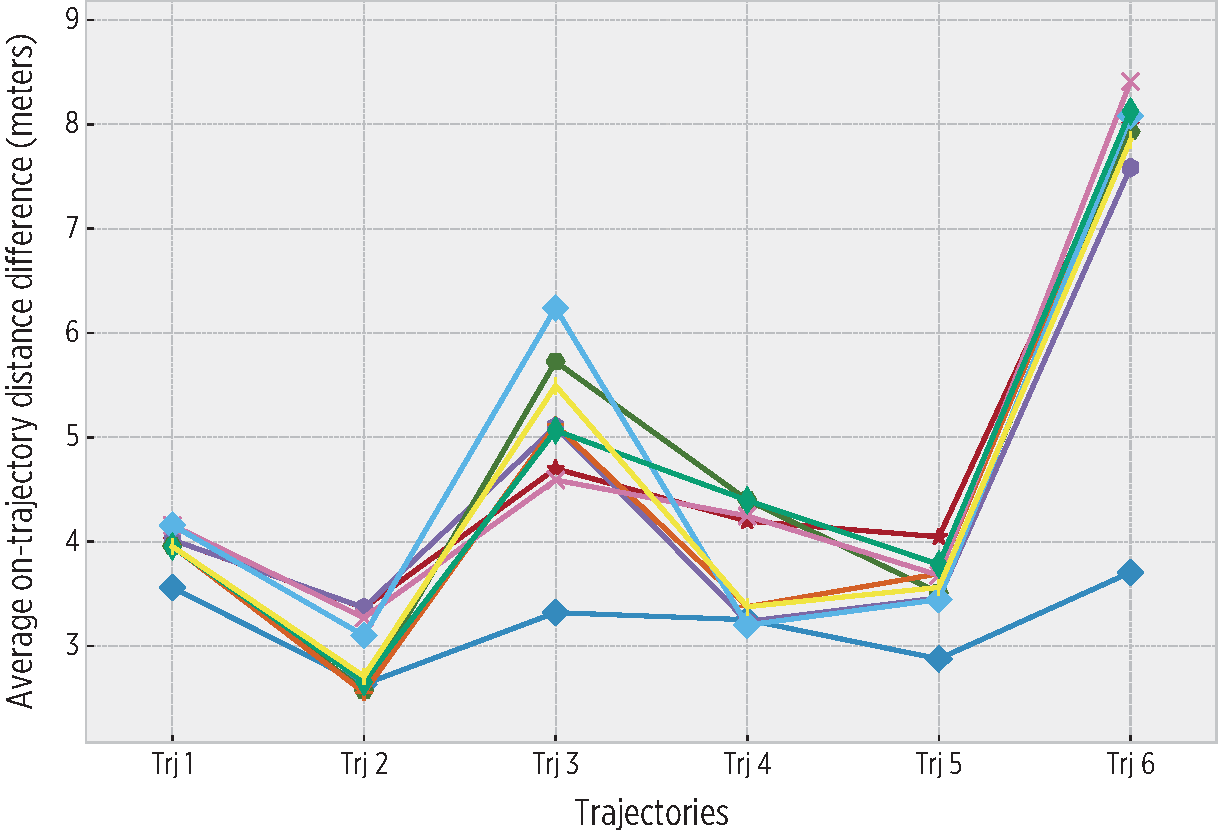
\includegraphics[width=\textwidth]{vectors/exp-4-on-trajectory-distance-for-slides-v2}
%   \captionof{figure}{The average distance of equivalent trajectory segments during experimental trials. The values are enclosed within $2.5~m$ and $8.5~m$, with the 30 seconds sampling obtaining the lowest values in each trial.}
%   \par
% }
% \end{block}

% \end{column}

% \begin{column}[T]{0.5\textwidth}
% \begin{block}{\small \textbf{Overall reduction of location update requests}}
% {
%   \centering
%   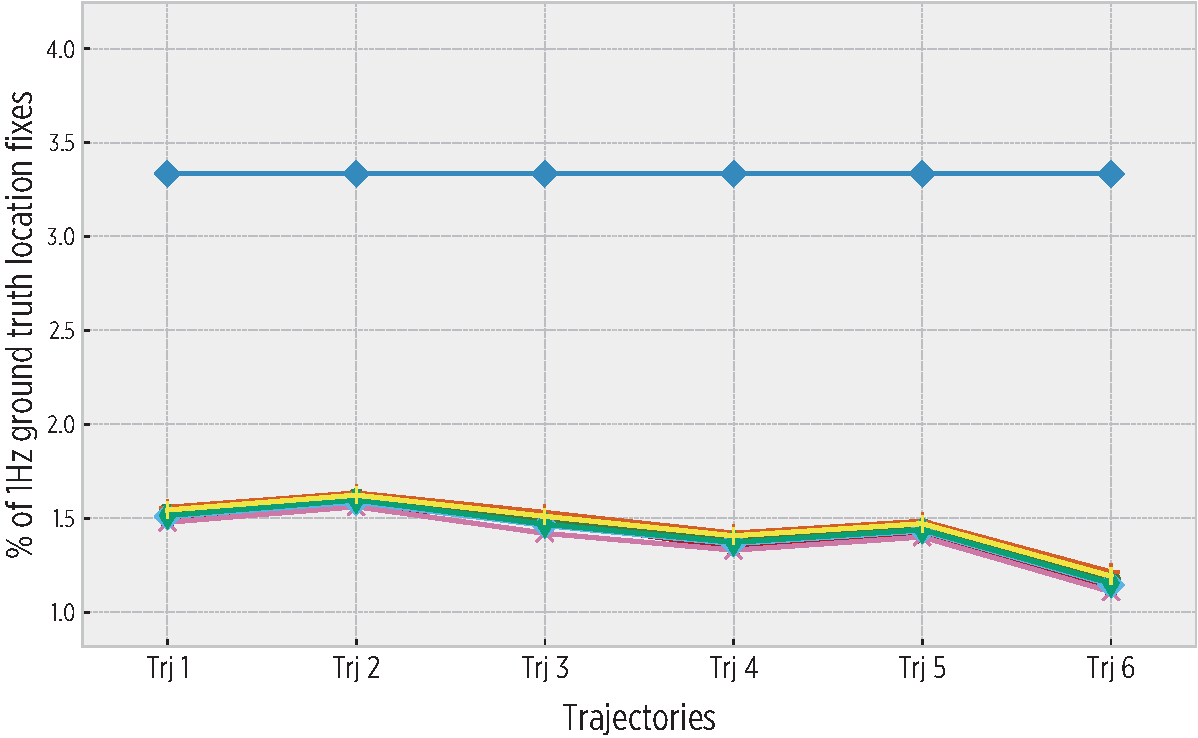
\includegraphics[width=\textwidth]{vectors/exp-4-location-requests-for-slides-v2}
%   \captionof{figure}{The proportion of location update requests employed by each experimental trial with respect to the corresponding $1~Hz$ ground truth trajectory. All of the parameter combinations outperform the 30 seconds sampling period, which provides a rough estimation of the energy savings that the system could achieve in on-device implementations.}
%   \par
% }
% \end{block}
% \end{column}
% \end{columns}
% \end{frame}

% \begin{frame}[noframenumbering]{Preliminary experimentation}{Energy saving expectations of on-device stay points detection}
% \small
% % \vspace{-0.5cm}
% \begin{columns}
% \begin{column}{0.55\textwidth}
% \begin{block}{\small \textbf{Description}}
% \begin{itemize}
%   \item This experiment explored whether a smartphone could detect stay points by itself, and the energy savings of such implementation with respect of typical Mobile Cloud Computing (MCC) based solutions.
%   % \item Typical solutions implement a Mobile Cloud Computing (MCC) approach on which the smartphone only collects and offloads the processing to external servers.
% \end{itemize}
% \end{block}
% \end{column}

% \begin{column}{0.4\textwidth}
% \begin{table}
% \centering
% \renewcommand{\arraystretch}{0.8}
% \resizebox{0.95\textwidth}{!}{%
% \begin{tabular}{lll}
% \toprule
% \multirow{2}{*}{\textbf{Stay Points Detector}} & \textbf{Time threshold} ($\delta_{time}$): & $45~min$ \\
% \cmidrule[0.25pt]{2-3}
%  & \textbf{Distance threshold} ($\delta_{distance}$): & $500~m$ \\

% \cmidrule[0.25pt]{1-3}
% \textbf{Sampling periods}: & \multicolumn{2}{l}{30, 60, 90, 120, 150 seconds} \\
% \bottomrule
% \end{tabular}
% }
% \caption{Input parameters for the energy saving expectations of on-device stay points detection experiment.}
% \end{table}
% \end{column}
% \end{columns}

% \begin{figure}
%   \centering
%   \includegraphics[width=\columnwidth]{vectors/plot-energy-performance-r2-for-slides}
%   \caption{Energy performance comparison of on-device vs. MCC sample apps using different GPS sampling periods. Each of the on-device trials last longer than its corresponding remote implementation.}
% \end{figure}

% \end{frame}


% \begin{frame}[noframenumbering]{Preliminary experimentation}{Energy consumption of fixed-sampling periods: Results}
% \vspace{-0.4cm}
% {
%   \centering
%   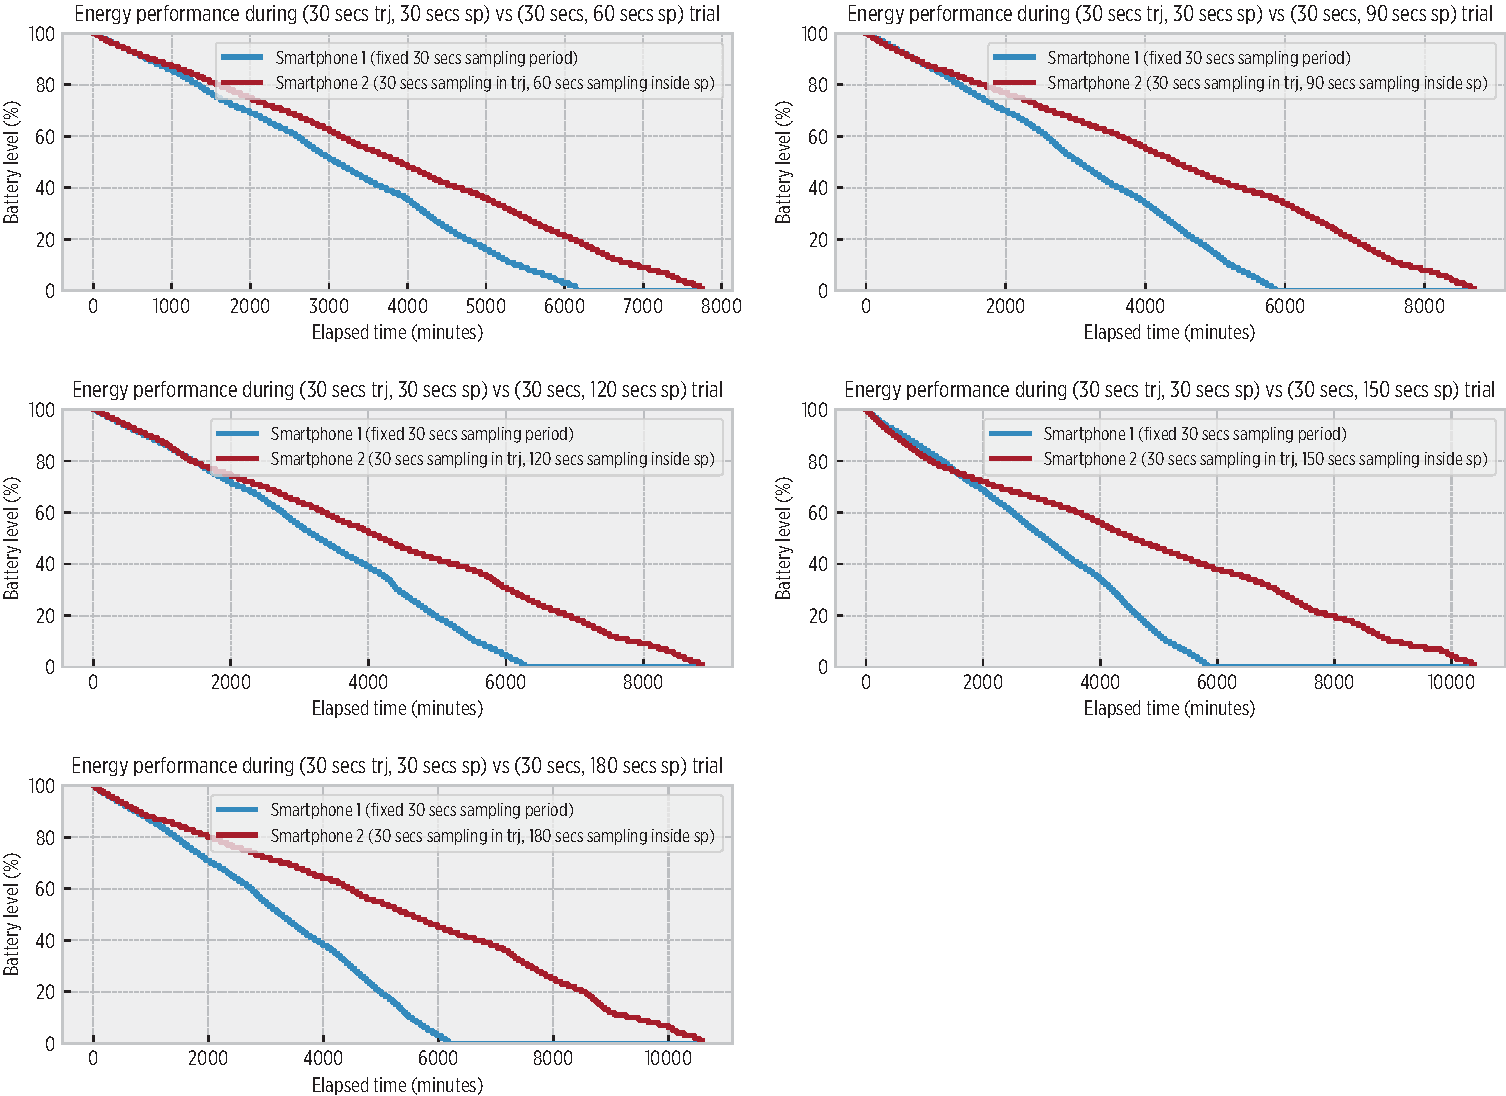
\includegraphics[width=0.85\textwidth]{vectors/exp-6-energy-burnout}
%   \captionof{figure}{Energy performance of a fixed 30 seconds sampling versus a basic sampling adaptation consisting in a 30 seconds sampling in trajectory mode and a slower sampling rate during stay point mode. The separation between the lines in each plot starts after the system learns the stay points with the largest weight in user mobility (home and work places).}
%   \par
% }
% \end{frame}


% \begin{frame}[noframenumbering]{Preliminary experimentation}{Energy consumption of fixed-sampling periods: Results}
% \vspace{-0.4cm}
% {
%   \centering
%   %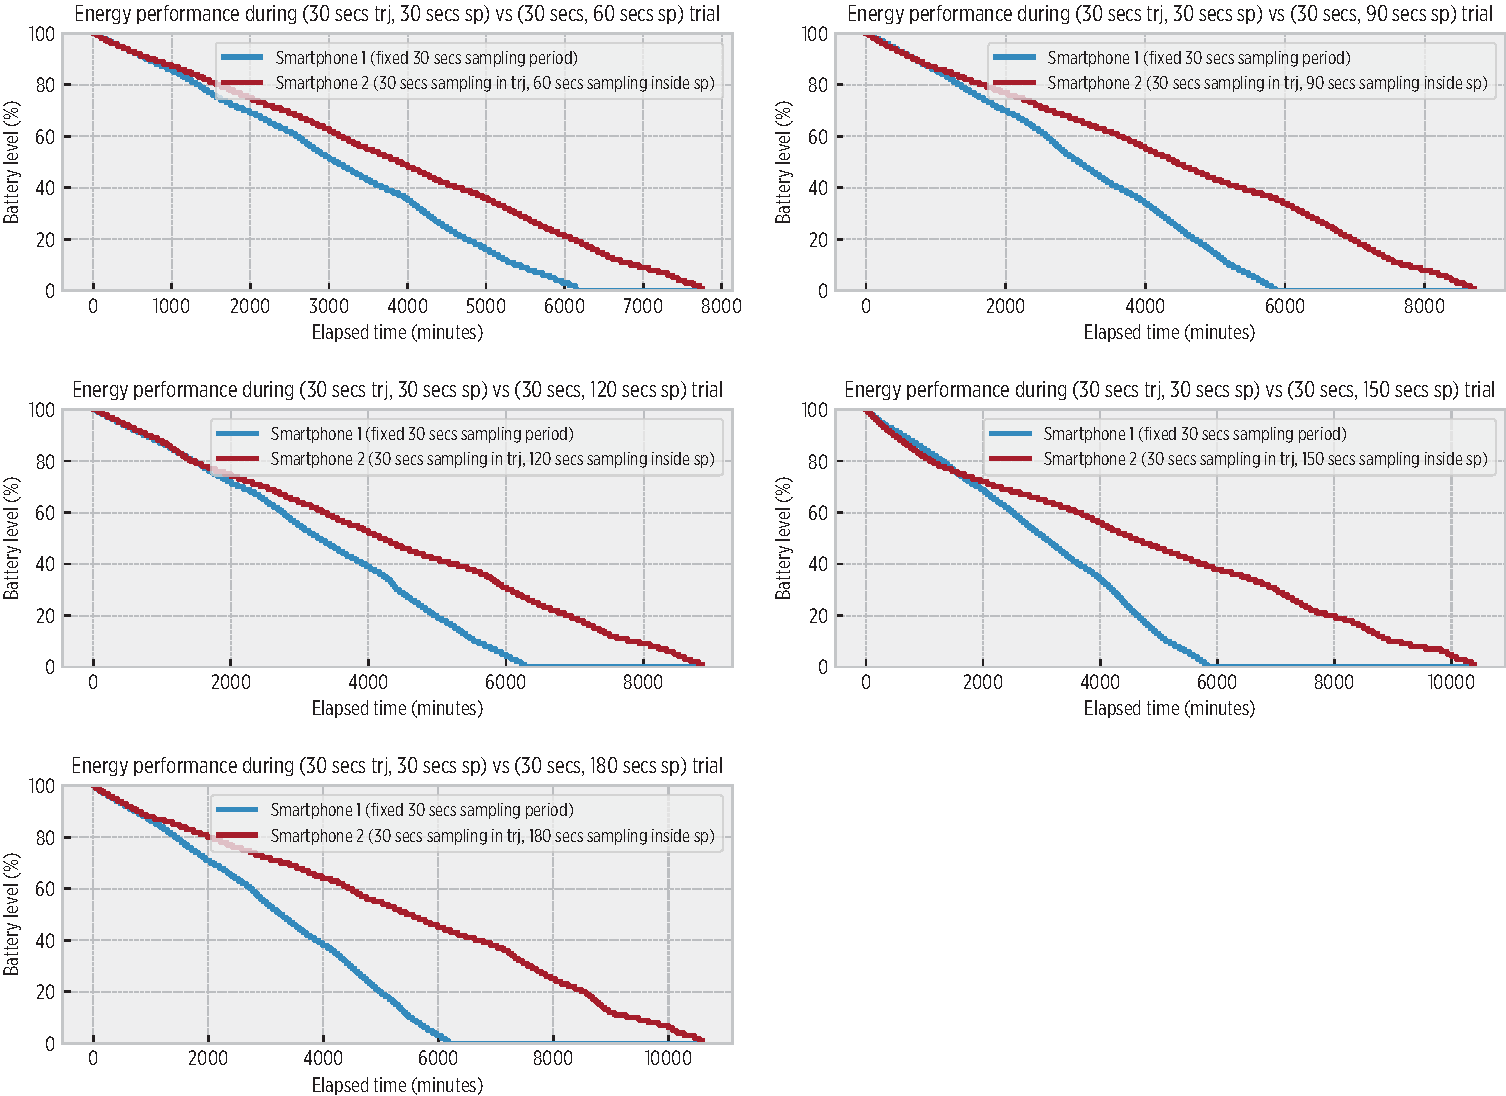
\includegraphics[width=0.85\textwidth]{vectors/exp-6-energy-burnout}
%   %\captionof{figure}{Energy performance of a fixed 30 seconds sampling versus a basic sampling adaptation consisting in a 30 seconds sampling in trajectory mode and a slower sampling rate during stay point mode. The separation between the lines in each plot starts after the system learns the stay points with the largest weight in user mobility (home and work places).}
%   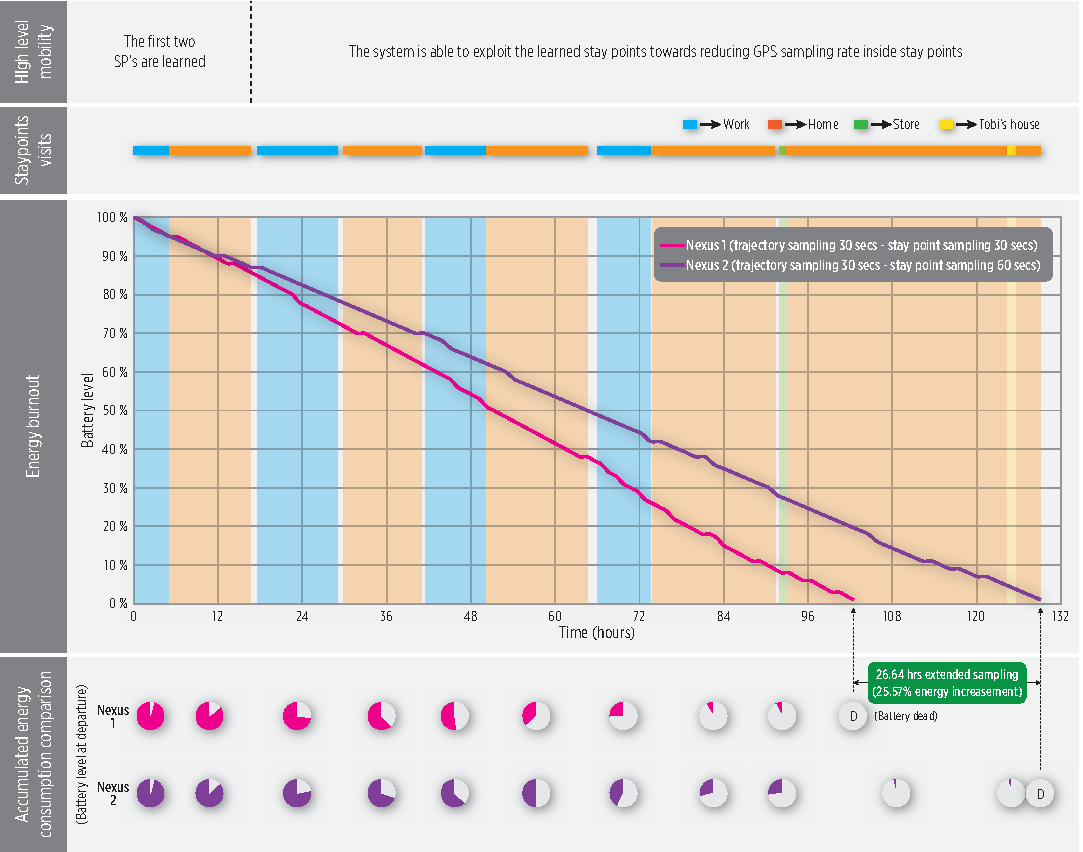
\includegraphics[width=0.8\textwidth]{vectors/energy-results-v2}
%   \captionof{figure}{Energy performance obtained by the CDS along the mobility described by user (trial corresponding to the 30 seconds in trajectory and 60 seconds in stay point sampling).}
%   \par
% }
% \end{frame}

% \begin{frame}[noframenumbering]{Preliminary experimentation}{Energy consumption of fixed-sampling periods: Results}
% \begin{figure}
%   % 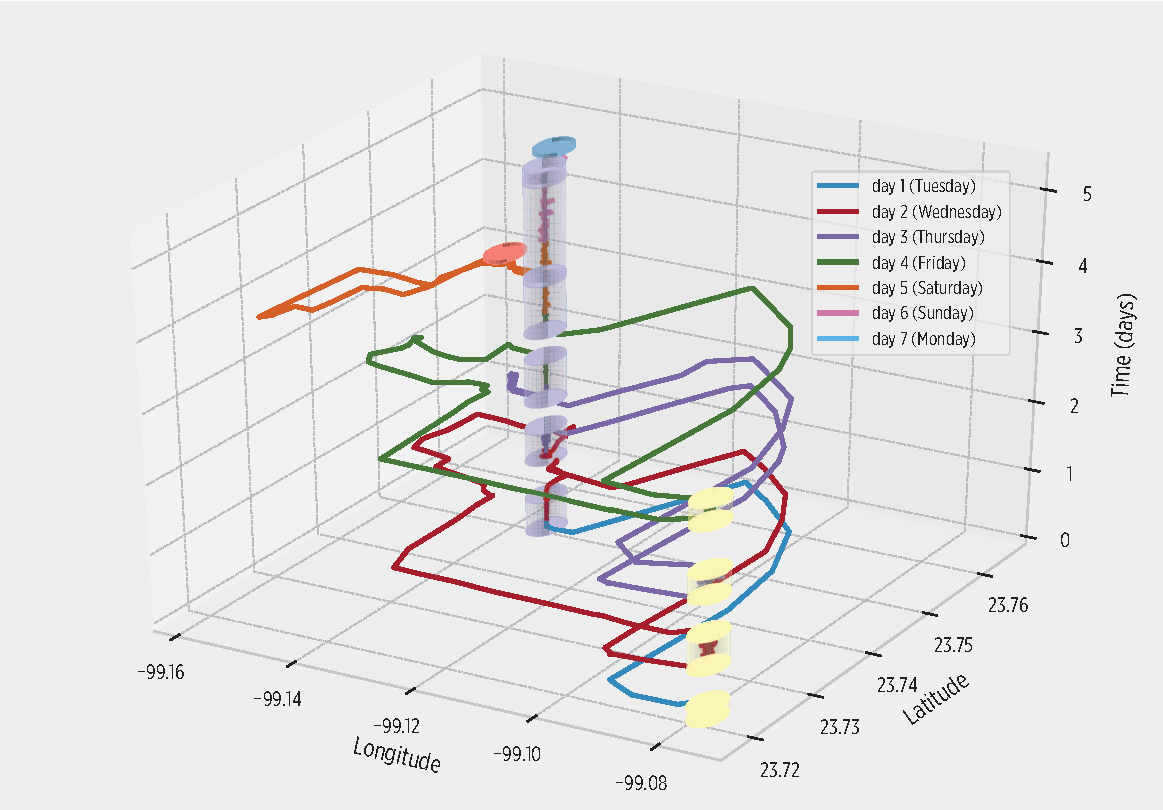
\includegraphics[width=0.8\textwidth]{vectors/exp-6-map-trj-4-adaptive-sampling-60-sp}
%   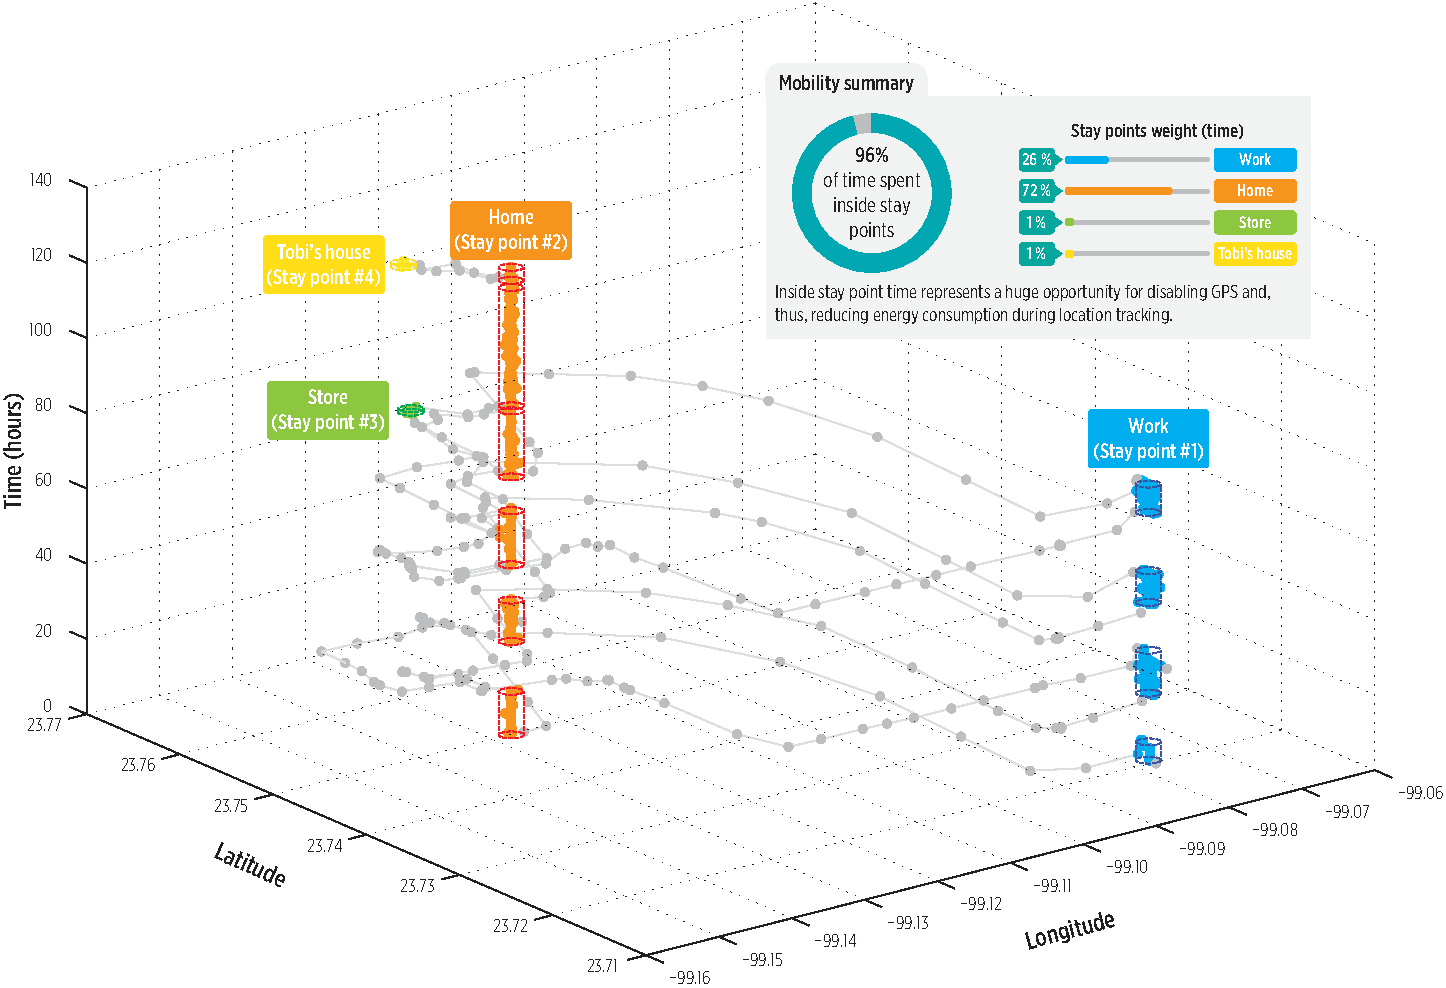
\includegraphics[width=0.85\textwidth]{vectors/stay-points-as-3d-v2}
%   \caption{The stay points and visits identified by the system, as well as the mobility summary obtained from such information (trial corresponding to the 30 seconds in trajectory and 60 seconds in stay point sampling).}
% %  \caption{The information autonomously learned by the STM during the trial corresponding to the 30 seconds in trajectory and 60 seconds in stay point sampling scheme. The height of cylinders corresponds with the stay time during each stay point visit.}
% \end{figure}
% \end{frame}
